
% LaTeX Beamer file automatically generated from DocOnce
% https://github.com/doconce/doconce

%-------------------- begin beamer-specific preamble ----------------------

\documentclass{beamer}

\usetheme{red_plain}
\usecolortheme{default}

% turn off the almost invisible, yet disturbing, navigation symbols:
\setbeamertemplate{navigation symbols}{}

% Examples on customization:
%\usecolortheme[named=RawSienna]{structure}
%\usetheme[height=7mm]{Rochester}
%\setbeamerfont{frametitle}{family=\rmfamily,shape=\itshape}
%\setbeamertemplate{items}[ball]
%\setbeamertemplate{blocks}[rounded][shadow=true]
%\useoutertheme{infolines}
%
%\usefonttheme{}
%\useinntertheme{}
%
%\setbeameroption{show notes}
%\setbeameroption{show notes on second screen=right}

% fine for B/W printing:
%\usecolortheme{seahorse}

\usepackage{pgf}
\usepackage{graphicx}
\usepackage{epsfig}
\usepackage{relsize}

\usepackage{fancybox}  % make sure fancybox is loaded before fancyvrb

\usepackage{fancyvrb}
\usepackage{minted} % requires pygments and latex -shell-escape filename
%\usepackage{anslistings}
%\usepackage{listingsutf8}

\usepackage{amsmath,amssymb,bm}
%\usepackage[latin1]{inputenc}
\usepackage[T1]{fontenc}
\usepackage[utf8]{inputenc}
\usepackage{colortbl}
\usepackage[english]{babel}
\usepackage{tikz}
\usepackage{framed}
% Use some nice templates
\beamertemplatetransparentcovereddynamic

% --- begin table of contents based on sections ---
% Delete this, if you do not want the table of contents to pop up at
% the beginning of each section:
% (Only section headings can enter the table of contents in Beamer
% slides generated from DocOnce source, while subsections are used
% for the title in ordinary slides.)
\AtBeginSection[]
{
  \begin{frame}<beamer>[plain]
  \frametitle{}
  %\frametitle{Outline}
  \tableofcontents[currentsection]
  \end{frame}
}
% --- end table of contents based on sections ---

% If you wish to uncover everything in a step-wise fashion, uncomment
% the following command:

%\beamerdefaultoverlayspecification{<+->}

\newcommand{\shortinlinecomment}[3]{\note{\textbf{#1}: #2}}
\newcommand{\longinlinecomment}[3]{\shortinlinecomment{#1}{#2}{#3}}

\definecolor{linkcolor}{rgb}{0,0,0.4}
\hypersetup{
    colorlinks=true,
    linkcolor=linkcolor,
    urlcolor=linkcolor,
    pdfmenubar=true,
    pdftoolbar=true,
    bookmarksdepth=3
    }
\setlength{\parskip}{0pt}  % {1em}

\newenvironment{doconceexercise}{}{}
\newcounter{doconceexercisecounter}
\newenvironment{doconce:movie}{}{}
\newcounter{doconce:movie:counter}

\newcommand{\subex}[1]{\noindent\textbf{#1}}  % for subexercises: a), b), etc

\logo{{\tiny \copyright\ 1999-2024, Morten Hjorth-Jensen. Released under CC Attribution-NonCommercial 4.0 license}}

%-------------------- end beamer-specific preamble ----------------------

% Add user's preamble




% insert custom LaTeX commands...

\raggedbottom
\makeindex

%-------------------- end preamble ----------------------

\begin{document}

% matching end for #ifdef PREAMBLE

\newcommand{\exercisesection}[1]{\subsection*{#1}}



% ------------------- main content ----------------------



% ----------------- title -------------------------

\title{Mathematics of discriminative and generative deep learning, from deep neural networks to diffusion models}

% ----------------- author(s) -------------------------

\author{Morten Hjorth-Jensen\inst{1,2}}
\institute{Department of Physics and Center for Computing in Science Education, University of Oslo, Norway\inst{1}
\and
Department of Physics and Astronomy and Facility for Rare Isotope Beams, Michigan State University, East Lansing, Michigan, USA\inst{2}}
% ----------------- end author(s) -------------------------

\date{STREAMLINE meeting, May 9-10, MSU, 2024
% <optional titlepage figure>
\ \\ 
{\tiny \copyright\ 1999-2024, Morten Hjorth-Jensen. Released under CC Attribution-NonCommercial 4.0 license}
}

\begin{frame}[plain,fragile]
\titlepage
\end{frame}

\begin{frame}[plain,fragile]
\frametitle{Types of machine learning}

\begin{block}{}
The approaches to machine learning are many, but are often split into two main categories. 
In \emph{supervised learning} we know the answer to a problem,
and let the computer deduce the logic behind it. On the other hand, \emph{unsupervised learning}
is a method for finding patterns and relationship in data sets without any prior knowledge of the system.

An emerging  third category is  \emph{reinforcement learning}. This is a paradigm 
of learning inspired by behavioural psychology, where learning is achieved by trial-and-error, 
solely from rewards and punishment.
\end{block}
\end{frame}

\begin{frame}[plain,fragile]
\frametitle{Main categories}

\begin{block}{}
Another way to categorize machine learning tasks is to consider the desired output of a system.
Some of the most common tasks are:

\begin{itemize}
  \item Classification: Outputs are divided into two or more classes. The goal is to   produce a model that assigns inputs into one of these classes. An example is to identify  digits based on pictures of hand-written ones. Classification is typically supervised learning.

  \item Regression: Finding a functional relationship between an input data set and a reference data set.   The goal is to construct a function that maps input data to continuous output values.

  \item Clustering: Data are divided into groups with certain common traits, without knowing the different groups beforehand.  It is thus a form of unsupervised learning.
\end{itemize}

\noindent
\end{block}
\end{frame}

\begin{frame}[plain,fragile]
\frametitle{Machine learning. A simple perspective on the interface between ML and Physics}

\vspace{6mm}

% inline figure
\centerline{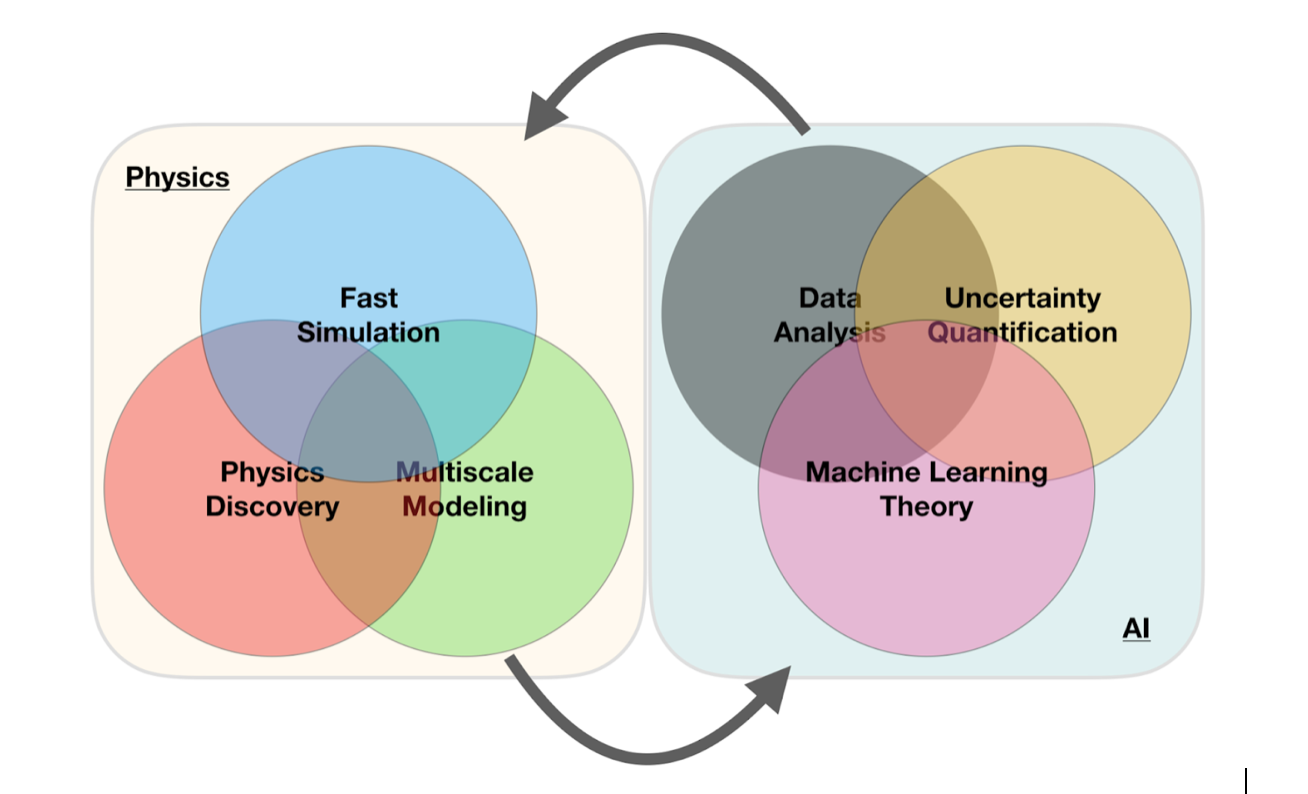
\includegraphics[width=1.0\linewidth]{figures/mlimage.png}}

\vspace{6mm}
\end{frame}

\begin{frame}[plain,fragile]
\frametitle{ML in Nuclear  Physics (or any field in physics)}

\vspace{6mm}

% inline figure
\centerline{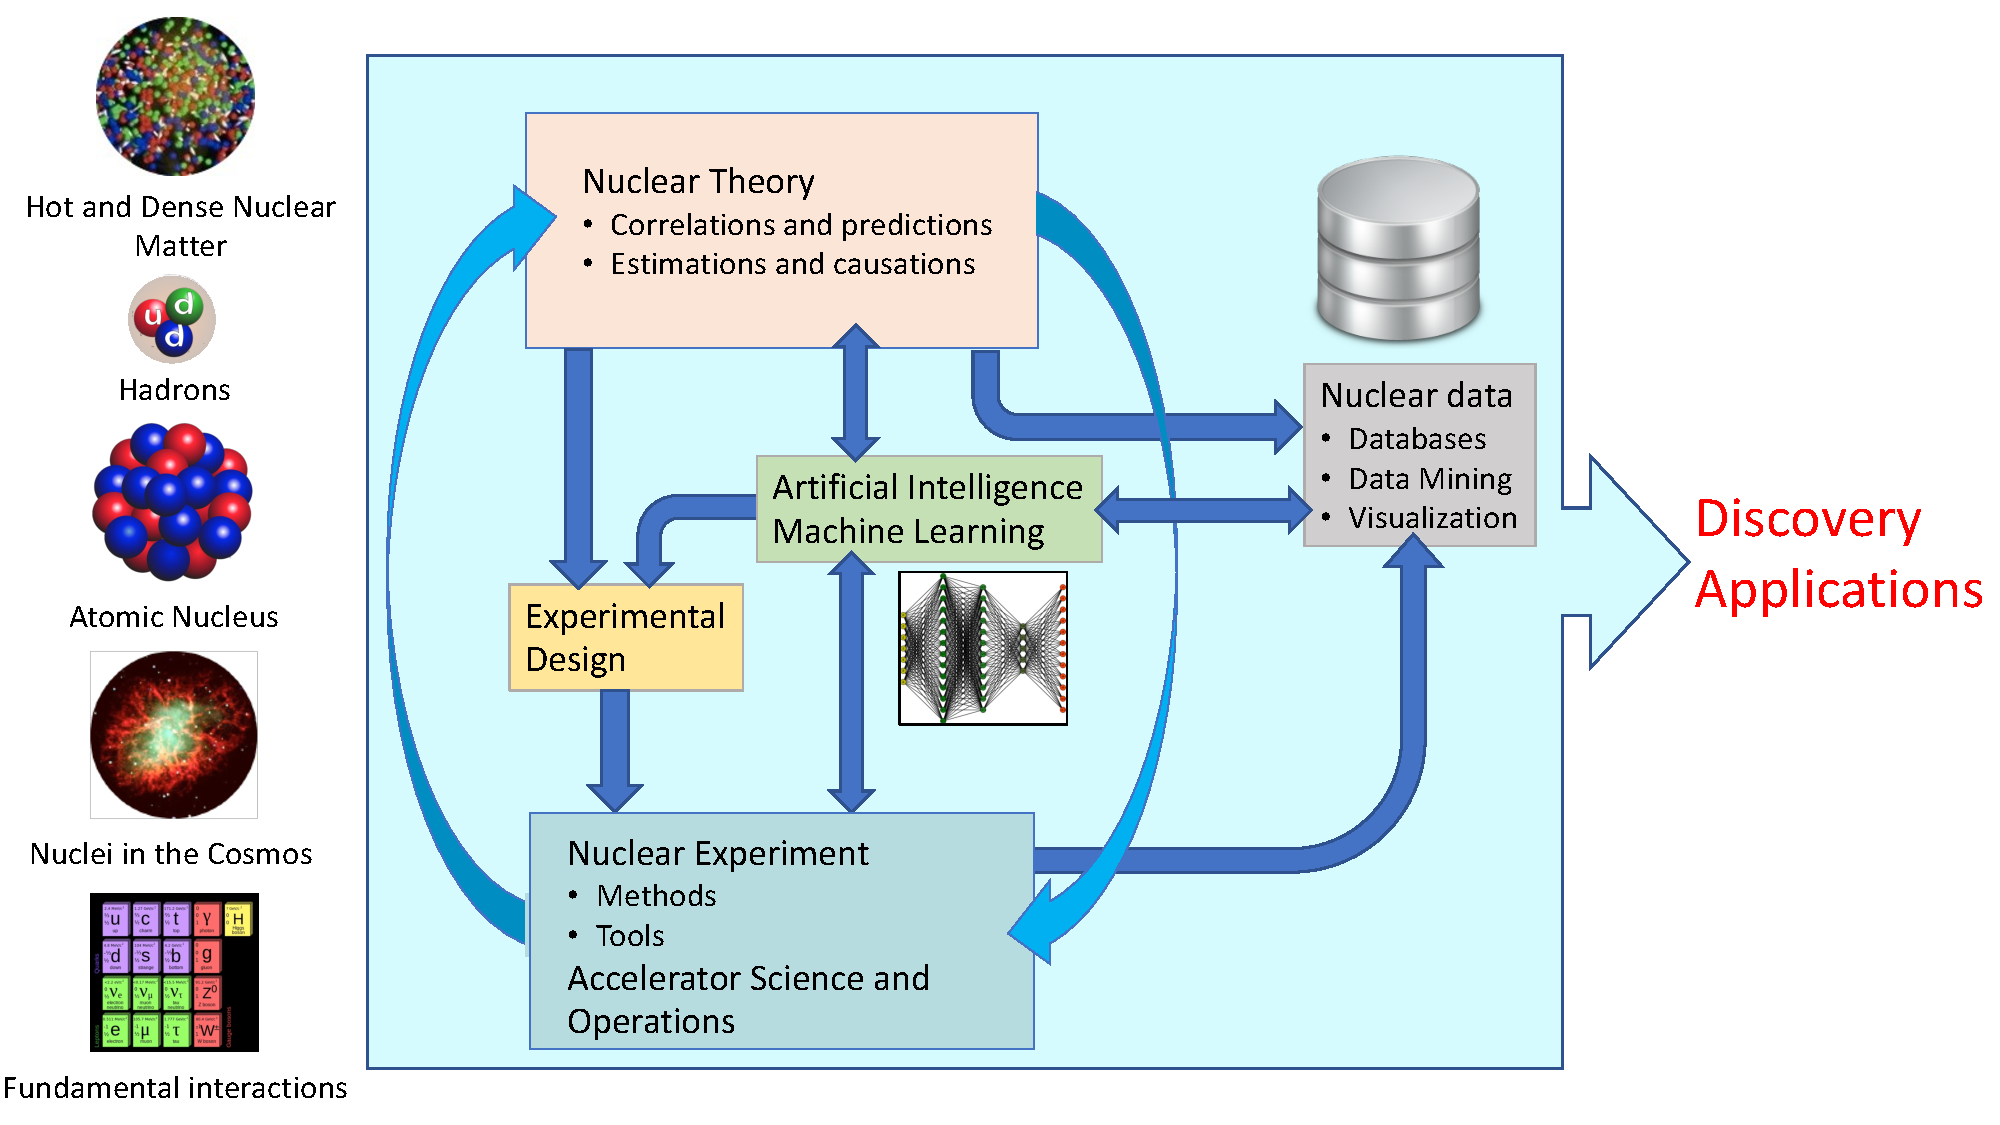
\includegraphics[width=1.0\linewidth]{figures/ML-NP.pdf}}

\vspace{6mm}
\end{frame}

\begin{frame}[plain,fragile]
\frametitle{The plethora  of machine learning algorithms/methods}

\begin{enumerate}
\item Deep learning: Neural Networks (NN), Convolutional NN, Recurrent NN, Boltzmann machines, autoencoders and variational autoencoders  and generative adversarial networks, stable diffusion and many more generative models

\item Bayesian statistics and Bayesian Machine Learning, Bayesian experimental design, Bayesian Regression models, Bayesian neural networks, Gaussian processes and much more

\item Dimensionality reduction (Principal component analysis), Clustering Methods and more

\item Ensemble Methods, Random forests, bagging and voting methods, gradient boosting approaches 

\item Linear and logistic regression, Kernel methods, support vector machines and more

\item Reinforcement Learning; Transfer Learning and more 
\end{enumerate}

\noindent
\end{frame}

\begin{frame}[plain,fragile]
\frametitle{What Is Generative Modeling?}

Generative modeling can be broadly defined as follows:

Generative modeling is a branch of machine learning that involves
training a model to produce new data that is similar to a given
dataset.

What does this mean in practice? Suppose we have a dataset containing
photos of horses. We can train a generative model on this dataset to
capture the rules that govern the complex relationships between pixels
in images of horses. Then we can sample from this model to create
novel, realistic images of horses that did not exist in the original
dataset.
\end{frame}

\begin{frame}[plain,fragile]
\frametitle{Example of generative modeling, \href{{https://www.oreilly.com/library/view/generative-deep-learning/9781098134174/ch01.html}}{taken from Generative Deep Learning by David Foster}}

\vspace{6mm}

% inline figure
\centerline{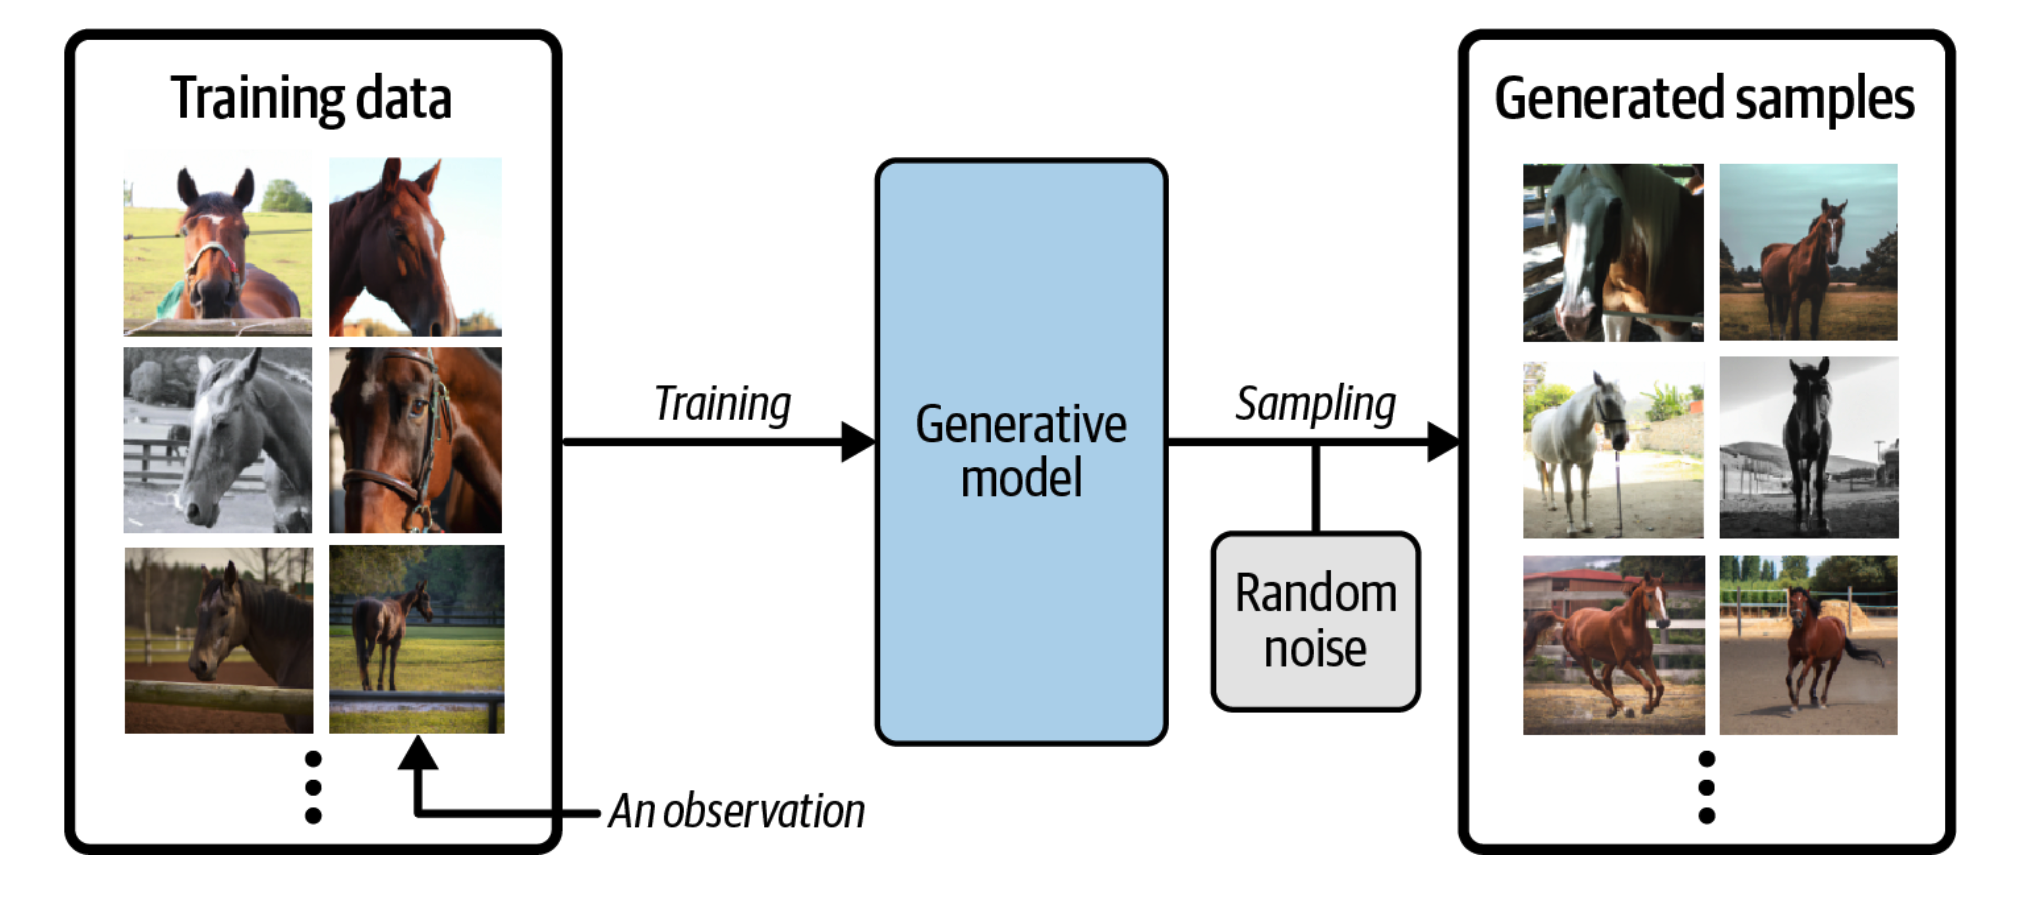
\includegraphics[width=1.0\linewidth]{figures/generativelearning.png}}

\vspace{6mm}
\end{frame}

\begin{frame}[plain,fragile]
\frametitle{Generative Modeling}

In order to build a generative model, we require a dataset consisting
of many examples of the entity we are trying to generate. This is
known as the training data, and one such data point is called an
observation.

Each observation consists of many features. For an image generation
problem, the features are usually the individual pixel values; for a
text generation problem, the features could be individual words or
groups of letters. It is our goal to build a model that can generate
new sets of features that look as if they have been created using the
same rules as the original data. Conceptually, for image generation
this is an incredibly difficult task, considering the vast number of
ways that individual pixel values can be assigned and the relatively
tiny number of such arrangements that constitute an image of the
entity we are trying to generate.
\end{frame}

\begin{frame}[plain,fragile]
\frametitle{Generative Versus Discriminative Modeling}

In order to truly understand what generative modeling aims to achieve
and why this is important, it is useful to compare it to its
counterpart, discriminative modeling. If you have studied machine
learning, most problems you will have faced will have most likely been
discriminative in nature.
\end{frame}

\begin{frame}[plain,fragile]
\frametitle{Example of discriminative modeling, \href{{https://www.oreilly.com/library/view/generative-deep-learning/9781098134174/ch01.html}}{taken from Generative Deeep Learning by David Foster}}

\vspace{6mm}

% inline figure
\centerline{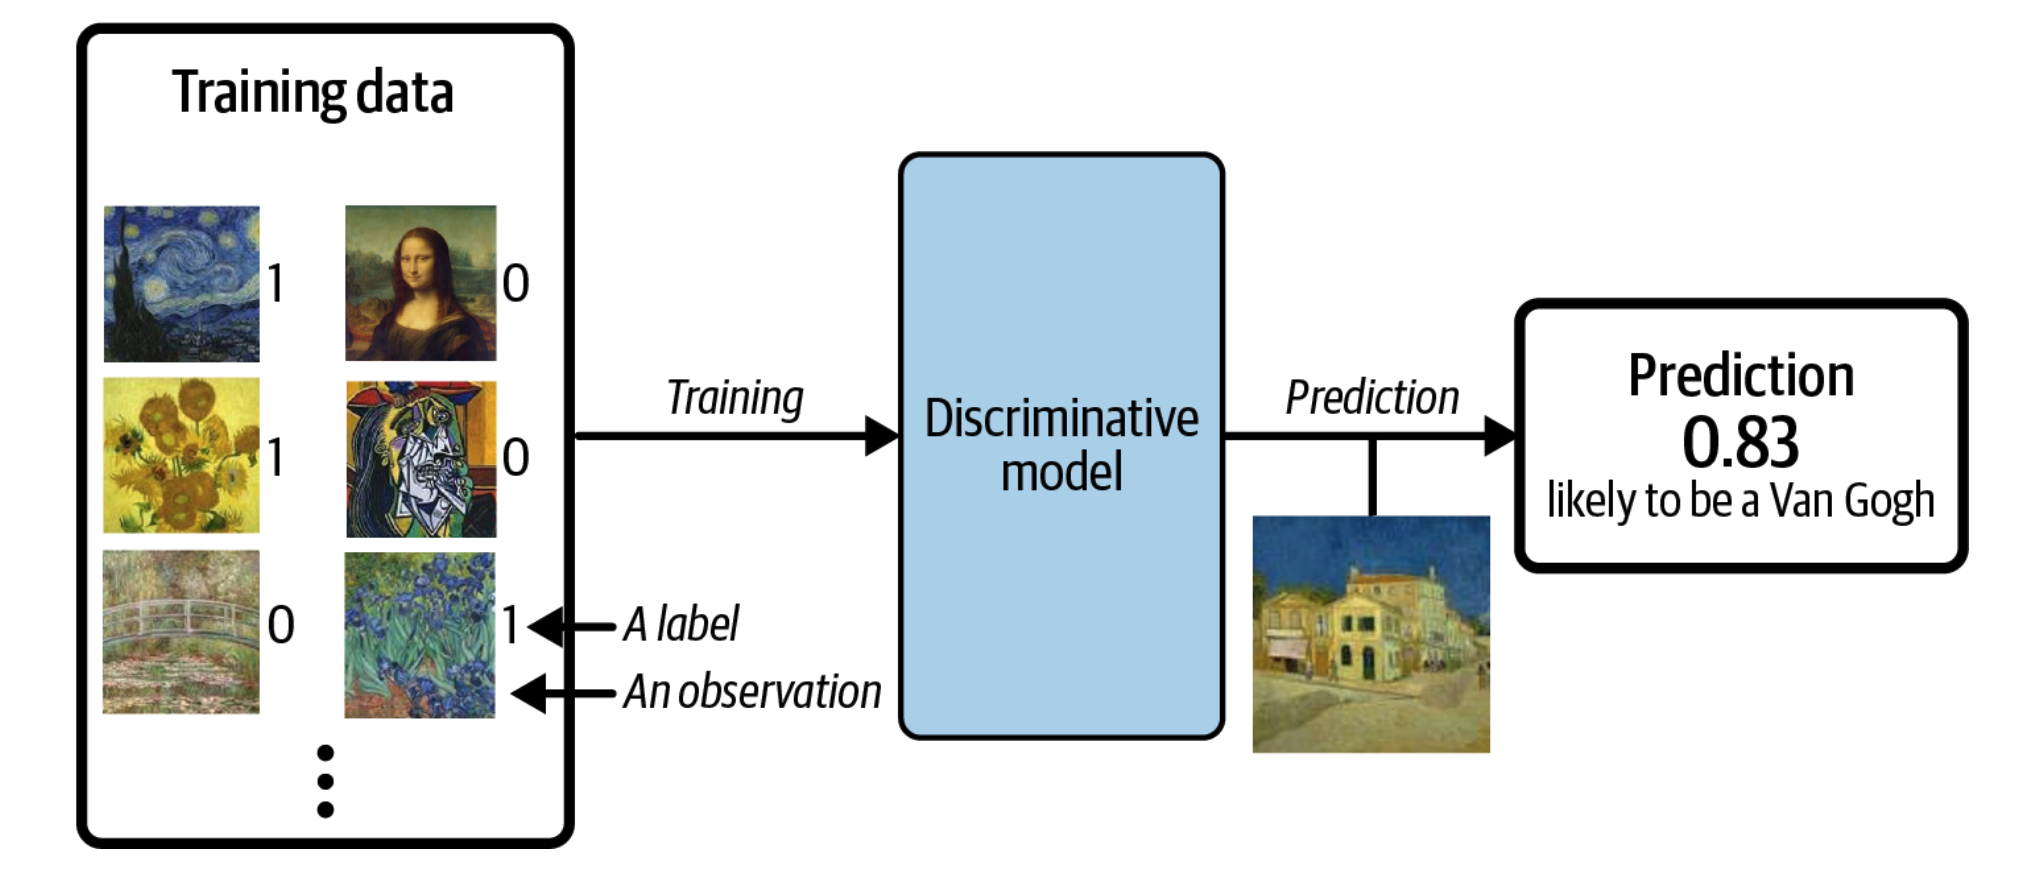
\includegraphics[width=1.0\linewidth]{figures/standarddeeplearning.png}}

\vspace{6mm}
\end{frame}

\begin{frame}[plain,fragile]
\frametitle{Discriminative Modeling}

When performing discriminative modeling, each observation in the
training data has a label. For a binary classification problem such as
our data could be labeled as ones and zeros. Our model then learns how to
discriminate between these two groups and outputs the probability that
a new observation has label 1 or 0

In contrast, generative modeling doesn’t require the dataset to be
labeled because it concerns itself with generating entirely new
data (for example an image), rather than trying to predict a label for say  a given image.
\end{frame}

\begin{frame}[plain,fragile]
\frametitle{Taxonomy of generative deep learning, \href{{https://www.oreilly.com/library/view/generative-deep-learning/9781098134174/ch01.html}}{taken from Generative Deep Learning by David Foster}}

\vspace{6mm}

% inline figure
\centerline{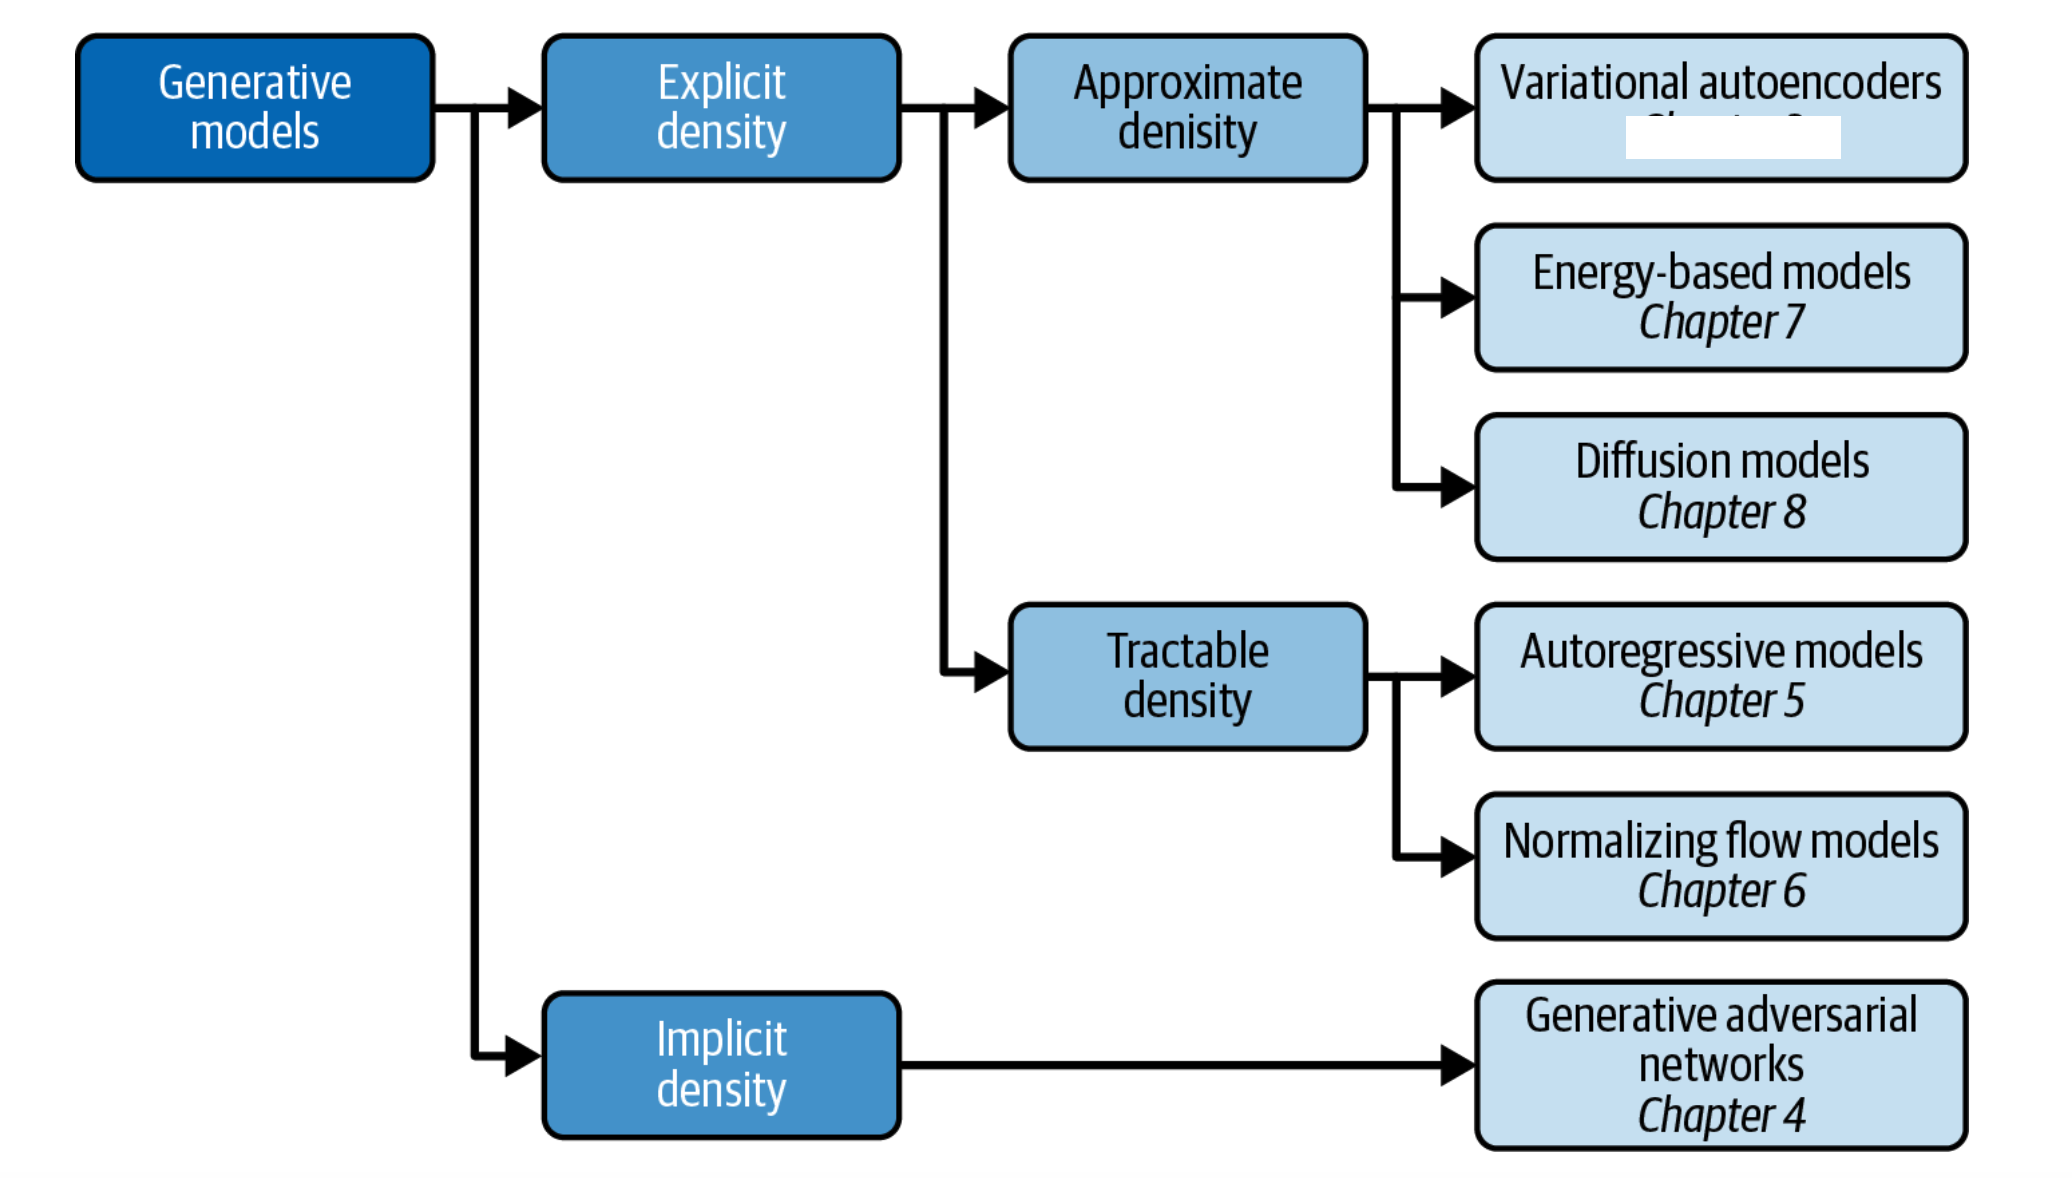
\includegraphics[width=1.0\linewidth]{figures/generativemodels.png}}

\vspace{6mm}
\end{frame}

\begin{frame}[plain,fragile]
\frametitle{Good books with hands-on material and codes}

\begin{block}{}
\begin{itemize}
\item \href{{https://sebastianraschka.com/blog/2022/ml-pytorch-book.html}}{Sebastian Rashcka et al, Machine learning with Sickit-Learn and PyTorch}

\item \href{{https://www.oreilly.com/library/view/generative-deep-learning/9781098134174/ch01.html}}{David Foster, Generative Deep Learning with TensorFlow}

\item \href{{https://github.com/PacktPublishing/Hands-On-Generative-AI-with-Python-and-TensorFlow-2}}{Babcock and Gavras, Generative AI with Python and TensorFlow 2}
\end{itemize}

\noindent
\end{block}

All three books have GitHub sites from where  one can download all codes. A good and more general text (2016)
is Goodfellow, Bengio and Courville, \href{{https://www.deeplearningbook.org/}}{Deep Learning}
\end{frame}

\begin{frame}[plain,fragile]
\frametitle{More references}

\begin{block}{Reading on diffusion models }
\begin{enumerate}
\item A central paper is the one by Sohl-Dickstein et al, Deep Unsupervised Learning using Nonequilibrium Thermodynamics, \href{{https://arxiv.org/abs/1503.03585}}{\nolinkurl{https://arxiv.org/abs/1503.03585}}

\item See also Diederik P. Kingma, Tim Salimans, Ben Poole, Jonathan Ho, Variational Diffusion Models, \href{{https://arxiv.org/abs/2107.00630}}{\nolinkurl{https://arxiv.org/abs/2107.00630}}
\end{enumerate}

\noindent
\end{block}   

\begin{block}{and VAEs }
\begin{enumerate}
\item Calvin Luo \href{{https://calvinyluo.com/2022/08/26/diffusion-tutorial.html}}{\nolinkurl{https://calvinyluo.com/2022/08/26/diffusion-tutorial.html}}

\item An Introduction to Variational Autoencoders, by Kingma and Welling, see \href{{https://arxiv.org/abs/1906.02691}}{\nolinkurl{https://arxiv.org/abs/1906.02691}}
\end{enumerate}

\noindent
\end{block}
\end{frame}

\begin{frame}[plain,fragile]
\frametitle{What are the basic Machine Learning ingredients?}

\begin{block}{}
Almost every problem in ML and data science starts with the same ingredients:
\begin{itemize}
\item The dataset $\bm{x}$ (could be some observable quantity of the system we are studying)

\item A model which is a function of a set of parameters $\bm{\alpha}$ that relates to the dataset, say a likelihood  function $p(\bm{x}\vert \bm{\alpha})$ or just a simple model $f(\bm{\alpha})$

\item A so-called \textbf{loss/cost/risk} function $\mathcal{C} (\bm{x}, f(\bm{\alpha}))$ which allows us to decide how well our model represents the dataset. 
\end{itemize}

\noindent
We seek to minimize the function $\mathcal{C} (\bm{x}, f(\bm{\alpha}))$ by finding the parameter values which minimize $\mathcal{C}$. This leads to  various minimization algorithms. It may surprise many, but at the heart of all machine learning algortihms there is an optimization problem. 
\end{block}
\end{frame}

\begin{frame}[plain,fragile]
\frametitle{Low-level machine learning, the family of ordinary least squares methods}

Our data which we want to apply a machine learning method on, consist
of a set of inputs $\bm{x}^T=[x_0,x_1,x_2,\dots,x_{n-1}]$ and the
outputs we want to model $\bm{y}^T=[y_0,y_1,y_2,\dots,y_{n-1}]$.
We assume  that the output data can be represented (for a regression case) by a continuous function $f$
through
\[
\bm{y}=f(\bm{x})+\bm{\epsilon}.
\]
\end{frame}

\begin{frame}[plain,fragile]
\frametitle{Setting up the equations}

In linear regression we approximate the unknown function with another
continuous function $\tilde{\bm{y}}(\bm{x})$ which depends linearly on
some unknown parameters
$\bm{\theta}^T=[\theta_0,\theta_1,\theta_2,\dots,\theta_{p-1}]$.

The input data can be organized in terms of a so-called design matrix 
with an approximating function $\bm{\tilde{y}}$ 
\[
\bm{\tilde{y}}= \bm{X}\bm{\theta},
\]
\end{frame}

\begin{frame}[plain,fragile]
\frametitle{The objective/cost/loss function}

The  simplest approach is the mean squared error
\[
C(\bm{\Theta})=\frac{1}{n}\sum_{i=0}^{n-1}\left(y_i-\tilde{y}_i\right)^2=\frac{1}{n}\left\{\left(\bm{y}-\bm{\tilde{y}}\right)^T\left(\bm{y}-\bm{\tilde{y}}\right)\right\},
\]
or using the matrix $\bm{X}$ and in a more compact matrix-vector notation as
\[
C(\bm{\Theta})=\frac{1}{n}\left\{\left(\bm{y}-\bm{X}\bm{\theta}\right)^T\left(\bm{y}-\bm{X}\bm{\theta}\right)\right\}.
\]
This function represents one of many possible ways to define the so-called cost function.
\end{frame}

\begin{frame}[plain,fragile]
\frametitle{Training solution}

Optimizing with respect to the unknown parameters $\theta_j$ we get 
\[
\bm{X}^T\bm{y} = \bm{X}^T\bm{X}\bm{\theta},  
\]
and if the matrix $\bm{X}^T\bm{X}$ is invertible we have the optimal values
\[
\hat{\bm{\theta}} =\left(\bm{X}^T\bm{X}\right)^{-1}\bm{X}^T\bm{y}.
\]

We say we 'learn' the unknown parameters $\bm{\theta}$ from the last equation.
\end{frame}

\begin{frame}[plain,fragile]
\frametitle{Ridge and LASSO Regression}

Our optimization problem is
\[
{\displaystyle \min_{\bm{\theta}\in {\mathbb{R}}^{p}}}\frac{1}{n}\left\{\left(\bm{y}-\bm{X}\bm{\theta}\right)^T\left(\bm{y}-\bm{X}\bm{\theta}\right)\right\}.
\]
or we can state it as
\[
{\displaystyle \min_{\bm{\theta}\in
{\mathbb{R}}^{p}}}\frac{1}{n}\sum_{i=0}^{n-1}\left(y_i-\tilde{y}_i\right)^2=\frac{1}{n}\vert\vert \bm{y}-\bm{X}\bm{\theta}\vert\vert_2^2,
\]
where we have used the definition of  a norm-2 vector, that is
\[
\vert\vert \bm{x}\vert\vert_2 = \sqrt{\sum_i x_i^2}. 
\]
\end{frame}

\begin{frame}[plain,fragile]
\frametitle{From OLS to Ridge and Lasso}

By minimizing the above equation with respect to the parameters
$\bm{\theta}$ we could then obtain an analytical expression for the
parameters $\bm{\theta}$.  We can add a regularization parameter $\lambda$ by
defining a new cost function to be optimized, that is

\[
{\displaystyle \min_{\bm{\theta}\in
{\mathbb{R}}^{p}}}\frac{1}{n}\vert\vert \bm{y}-\bm{X}\bm{\theta}\vert\vert_2^2+\lambda\vert\vert \bm{\theta}\vert\vert_2^2
\]

which leads to the Ridge regression minimization problem where we
require that $\vert\vert \bm{\theta}\vert\vert_2^2\le t$, where $t$ is
a finite number larger than zero. We do not include such a constraints in the discussions here.
\end{frame}

\begin{frame}[plain,fragile]
\frametitle{Lasso regression}

Defining

\[
C(\bm{X},\bm{\theta})=\frac{1}{n}\vert\vert \bm{y}-\bm{X}\bm{\theta}\vert\vert_2^2+\lambda\vert\vert \bm{\theta}\vert\vert_1,
\]
we have a new optimization equation
\[
{\displaystyle \min_{\bm{\theta}\in
{\mathbb{R}}^{p}}}\frac{1}{n}\vert\vert \bm{y}-\bm{X}\bm{\theta}\vert\vert_2^2+\lambda\vert\vert \bm{\theta}\vert\vert_1
\]
which leads to Lasso regression. Lasso stands for least absolute shrinkage and selection operator. 
Here we have defined the norm-1 as 
\[
\vert\vert \bm{x}\vert\vert_1 = \sum_i \vert x_i\vert. 
\]
\end{frame}

\begin{frame}[plain,fragile]
\frametitle{Selected references}

\begin{block}{}
\begin{itemize}
\item \href{{https://arxiv.org/abs/1803.08823}}{Mehta et al.} and \href{{https://www.sciencedirect.com/science/article/pii/S0370157319300766?via%3Dihub}}{Physics Reports (2019)}.

\item \href{{https://link.aps.org/doi/10.1103/RevModPhys.91.045002}}{Machine Learning and the Physical Sciences by Carleo et al}

\item \href{{https://journals.aps.org/rmp/abstract/10.1103/RevModPhys.94.031003}}{Artificial Intelligence and Machine Learning in Nuclear Physics, Amber Boehnlein et al., Reviews Modern of Physics 94, 031003 (2022)} 

\item \href{{https://journals.aps.org/prresearch/pdf/10.1103/PhysRevResearch.5.033062}}{Dilute neutron star matter from neural-network quantum states by Fore et al, Physical Review Research 5, 033062 (2023)}

\item Neural-network quantum states for ultra-cold Fermi gases, Jane Kim et al, Nature Physics Communcication, in press, see \href{{https://doi.org/10.48550/arXiv.2305.08831}}{\nolinkurl{https://doi.org/10.48550/arXiv.2305.08831}}

\item \href{{https://doi.org/10.48550/arXiv.2305.07240}}{Message-Passing Neural Quantum States for the Homogeneous Electron Gas, Gabriel Pescia, Jane Kim et al.~arXiv.2305.07240,}

\item \href{{https://pdg.lbl.gov/2021/reviews/rpp2021-rev-machine-learning.pdf}}{Particle Data Group summary on ML methods}
\end{itemize}

\noindent
\end{block}
\end{frame}

\begin{frame}[plain,fragile]
\frametitle{Setting up the basic equations for neural networks}

Neural networks, in its so-called feed-forward form, where each
iterations contains a feed-forward stage and a back-propgagation
stage, consist of series of affine matrix-matrix and matrix-vector
multiplications. The unknown parameters (the so-called biases and
weights which deternine the architecture of a neural network), are
uptaded iteratively using the so-called back-propagation algorithm.
This algorithm corresponds to the so-called reverse mode of the
automatic differentation algorithm. These algorithms will be discussed
in more detail below.

We start however first with the  definitions of the various variables which make up a neural network.
\end{frame}

\begin{frame}[plain,fragile]
\frametitle{Overarching view of a neural network}

The architecture of a neural network defines our model. This model
aims at describing some function $f(\bm{x}$ which aims at describing
some final result (outputs or tagrget values) given a specific inpput
$\bm{x}$. Note that here $\bm{y}$ and $\bm{x}$ are not limited to be
vectors.

The architecture consists of
\begin{enumerate}
\item An input and an output layer where the input layer is defined by the inputs $\bm{x}$. The output layer produces the model ouput $\bm{\tilde{y}}$ which is compared with the target value $\bm{y}$

\item A given number of hidden layers and neurons/nodes/units for each layer (this may vary)

\item A given activation function $\sigma(\bm{z})$ with arguments $\bm{z}$ to be defined below. The activation functions may differ from layer to layer.

\item The last layer, normally called \textbf{output} layer has normally an activation function tailored to the specific problem

\item Finally we define a so-called cost or loss function which is used to gauge the quality of our model. 
\end{enumerate}

\noindent
\end{frame}

\begin{frame}[plain,fragile]
\frametitle{Illustration of a single perceptron model and a multilayer FFNN}

\begin{figure}[!ht]  % 
  \centerline{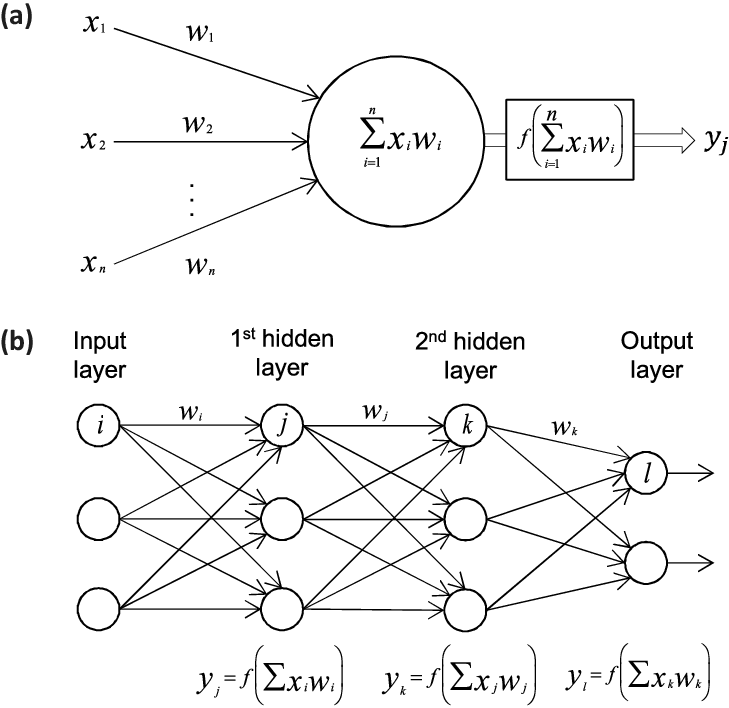
\includegraphics[width=0.7\linewidth]{figures/nns.png}}
  \caption{
  In a) we show a single perceptron model while in b) we dispay a network with two  hidden layers, an input layer and an output layer.
  }
\end{figure}
%\clearpage % flush figures
\end{frame}

\begin{frame}[plain,fragile]
\frametitle{The optimization problem}

The cost function is a function of the unknown parameters
$\bm{\Theta}$ where the latter is a container for all possible
parameters needed to define a neural network

If we are dealing with a regression task a typical cost/loss function
is the mean squared error
\[
C(\bm{\Theta})=\frac{1}{n}\left\{\left(\bm{y}-\bm{X}\bm{\theta}\right)^T\left(\bm{y}-\bm{X}\bm{\theta}\right)\right\}.
\]
This function represents one of many possible ways to define
the so-called cost function.
\end{frame}

\begin{frame}[plain,fragile]
\frametitle{Weights and biases}

For neural networks the parameters
$\bm{\Theta}$ are given by the so-called weights and biases (to be
defined below).

The weights are given by matrix elements $w_{ij}^{(l)}$ where the
superscript indicates the layer number. The biases are typically given
by vector elements representing each single node of a given layer,
that is $b_j^{(l)}$.
\end{frame}

\begin{frame}[plain,fragile]
\frametitle{Other ingredients of a neural network}

Having defined the architecture of a neural network, the optimization
of the cost function with respect to the parameters $\bm{\Theta}$,
involves the calculations of gradients and their optimization. The
gradients represent the derivatives of a multidimensional object and
are often approximated by various gradient methods, including
\begin{enumerate}
\item various quasi-Newton methods,

\item plain gradient descent (GD) with a constant learning rate $\eta$,

\item GD with momentum and other approximations to the learning rates such as
\begin{itemize}

  \item Adapative gradient (ADAgrad)

  \item Root mean-square propagation (RMSprop)

  \item Adaptive gradient with momentum (ADAM) and many other

\end{itemize}

\noindent
\item Stochastic gradient descent and various families of learning rate approximations
\end{enumerate}

\noindent
\end{frame}

\begin{frame}[plain,fragile]
\frametitle{Other parameters}

In addition to the above, there are often additional hyperparamaters
which are included in the setup of a neural network. These will be
discussed below.
\end{frame}

\begin{frame}[plain,fragile]
\frametitle{Why Feed Forward Neural Networks (FFNN)?}

According to the \emph{Universal approximation theorem}, a feed-forward
neural network with just a single hidden layer containing a finite
number of neurons can approximate a continuous multidimensional
function to arbitrary accuracy, assuming the activation function for
the hidden layer is a \textbf{non-constant, bounded and
monotonically-increasing continuous function}.
\end{frame}

\begin{frame}[plain,fragile]
\frametitle{Universal approximation theorem}

The universal approximation theorem plays a central role in deep
learning.  \href{{https://link.springer.com/article/10.1007/BF02551274}}{Cybenko (1989)} showed
the following:

\begin{block}{}
Let $\sigma$ be any continuous sigmoidal function such that
\[
\sigma(z) = \left\{\begin{array}{cc} 1 & z\rightarrow \infty\\ 0 & z \rightarrow -\infty \end{array}\right.
\]
Given a continuous and deterministic function $F(\bm{x})$ on the unit
cube in $d$-dimensions $F\in [0,1]^d$, $x\in [0,1]^d$ and a parameter
$\epsilon >0$, there is a one-layer (hidden) neural network
$f(\bm{x};\bm{\Theta})$ with $\bm{\Theta}=(\bm{W},\bm{b})$ and $\bm{W}\in
\mathbb{R}^{m\times n}$ and $\bm{b}\in \mathbb{R}^{n}$, for which
\[
\vert F(\bm{x})-f(\bm{x};\bm{\Theta})\vert < \epsilon \hspace{0.1cm} \forall \bm{x}\in[0,1]^d.
\]

\end{block}
\end{frame}

\begin{frame}[plain,fragile]
\frametitle{The approximation theorem in words}

\textbf{Any continuous function $y=F(\bm{x})$ supported on the unit cube in
$d$-dimensions can be approximated by a one-layer sigmoidal network to
arbitrary accuracy.}

\href{{https://www.sciencedirect.com/science/article/abs/pii/089360809190009T}}{Hornik (1991)} extended the theorem by letting any non-constant, bounded activation function to be included using that the expectation value
\[
\mathbb{E}[\vert F(\bm{x})\vert^2] =\int_{\bm{x}\in D} \vert F(\bm{x})\vert^2p(\bm{x})d\bm{x} < \infty.
\]
Then we have
\[
\mathbb{E}[\vert F(\bm{x})-f(\bm{x};\bm{\Theta})\vert^2] =\int_{\bm{x}\in D} \vert F(\bm{x})-f(\bm{x};\bm{\Theta})\vert^2p(\bm{x})d\bm{x} < \epsilon.
\]
\end{frame}

\begin{frame}[plain,fragile]
\frametitle{More on the general approximation theorem}

None of the proofs give any insight into the relation between the
number of of hidden layers and nodes and the approximation error
$\epsilon$, nor the magnitudes of $\bm{W}$ and $\bm{b}$.

Neural networks (NNs) have what we may call a kind of universality no matter what function we want to compute.

\begin{block}{}
It does not mean that an NN can be used to exactly compute any function. Rather, we get an approximation that is as good as we want. 
\end{block}
\end{frame}

\begin{frame}[plain,fragile]
\frametitle{Class of functions we can approximate}

\begin{block}{}
The class of functions that can be approximated are the continuous ones.
If the function $F(\bm{x})$ is discontinuous, it won't in general be possible to approximate it. However, an NN may still give an approximation even if we fail in some points.
\end{block}
\end{frame}

\begin{frame}[plain,fragile]
\frametitle{Simple example, fitting nuclear masses}

See example at \href{{https://github.com/CompPhysics/MachineLearning/blob/master/doc/pub/week34/ipynb/week34.ipynb}}{\nolinkurl{https://github.com/CompPhysics/MachineLearning/blob/master/doc/pub/week34/ipynb/week34.ipynb}}, and scroll down to nuclear masses.

And the recent article \href{{https://www.sciencedirect.com/science/article/pii/S0375947423001100}}{\nolinkurl{https://www.sciencedirect.com/science/article/pii/S0375947423001100}}
\end{frame}

\begin{frame}[plain,fragile]
\frametitle{First network example, simple percepetron with one input}

As yet another example we define now a simple perceptron model with
all quantities given by scalars. We consider only one input variable
$x$ and one target value $y$.  We define an activation function
$\sigma_1$ which takes as input

\[
z_1 = w_1x+b_1,
\]
where $w_1$ is the weight and $b_1$ is the bias. These are the
parameters we want to optimize.  The output is $a_1=\sigma(z_1)$ (see
graph from whiteboard notes). This output is then fed into the
\textbf{cost/loss} function, which we here for the sake of simplicity just
define as the squared error

\[
C(x;w_1,b_1)=\frac{1}{2}(a_1-y)^2.
\]
\end{frame}

\begin{frame}[plain,fragile]
\frametitle{Optimizing the parameters}

In setting up the feed forward and back propagation parts of the
algorithm, we need now the derivative of the various variables we want
to train.

We need
\[
\frac{\partial C}{\partial w_1} \hspace{0.1cm}\mathrm{and}\hspace{0.1cm}\frac{\partial C}{\partial b_1}. 
\]

Using the chain rule we find 
\[
\frac{\partial C}{\partial w_1}=\frac{\partial C}{\partial a_1}\frac{\partial a_1}{\partial z_1}\frac{\partial z_1}{\partial w_1}=(a_1-y)\sigma_1'x,
\]
and
\[
\frac{\partial C}{\partial b_1}=\frac{\partial C}{\partial a_1}\frac{\partial a_1}{\partial z_1}\frac{\partial z_1}{\partial b_1}=(a_1-y)\sigma_1',
\]
which we later will just define as
\[
\frac{\partial C}{\partial a_1}\frac{\partial a_1}{\partial z_1}=\delta_1.
\]
\end{frame}

\begin{frame}[plain,fragile]
\frametitle{Implementing the simple perceptron model}

In the example code here we implement the above equations (with explict
expressions for the derivatives) with just one input variable $x$ and
one output variable.  The target value $y=2x+1$ is a simple linear
function in $x$. Since this is a regression problem, we define the cost function to be proportional to the least squares error
\[
C(y,w_1,b_1)=\frac{1}{2}(a_1-y)^2,
\]
with $a_1$ the output from the network.





















































\begin{minted}[fontsize=\fontsize{9pt}{9pt},linenos=false,mathescape,baselinestretch=1.0,fontfamily=tt,xleftmargin=2mm]{python}
# import necessary packages
import numpy as np
import matplotlib.pyplot as plt

def feed_forward(x):
    # weighted sum of inputs to the output layer
    z_1 = x*output_weights + output_bias
    # Output from output node (one node only)
    # Here the output is equal to the input
    a_1 = z_1
    return a_1

def backpropagation(x, y):
    a_1 = feed_forward(x)
    # derivative of cost function
    derivative_cost = a_1 - y
    # the variable delta in the equations, note that output a_1 = z_1, its derivatives wrt z_o is thus 1
    delta_1 = derivative_cost
    # gradients for the output layer
    output_weights_gradient = delta_1*x
    output_bias_gradient = delta_1
    # The cost function is 0.5*(a_1-y)^2. This gives a measure of the error for each iteration
    return output_weights_gradient, output_bias_gradient

# ensure the same random numbers appear every time
np.random.seed(0)
# Input variable
x = 4.0
# Target values
y = 2*x+1.0

# Defining the neural network
n_inputs = 1
n_outputs = 1
# Initialize the network
# weights and bias in the output layer
output_weights = np.random.randn()
output_bias = np.random.randn()

# implementing a simple gradient descent approach with fixed learning rate
eta = 0.01
for i in range(40):
    # calculate gradients from back propagation
    derivative_w1, derivative_b1 = backpropagation(x, y)
    # update weights and biases
    output_weights -= eta * derivative_w1
    output_bias -= eta * derivative_b1
# our final prediction after training
ytilde = output_weights*x+output_bias
print(0.5*((ytilde-y)**2))


\end{minted}

Running this code gives us an acceptable results after some 40-50 iterations. Note that the results depend on the value of the learning rate.
\end{frame}

\begin{frame}[plain,fragile]
% No title on this slide

% --- begin exercise ---
\begin{doconceexercise}
\refstepcounter{doconceexercisecounter}

\exercisesection{Exercise \thedoconceexercisecounter: Extensions to the above code}
                             

Feel free to add more input nodes and weights to the above
code. Furthermore, try to increase the amount of input and
target/output data. Try also to perform calculations for more values
of the learning rates. Feel free to add either hyperparameters with an
$l_1$ norm or an $l_2$ norm and discuss your results.

You could also try to change the function $f(x)=y$ from a linear polynomial in $x$ to a higher-order polynomial.
Comment your results.

\textbf{Hint}: Increasing the number of input variables and input nodes requires a rewrite of the input data in terms of a matrix. You need to figure out the correct dimensionalities.

\end{doconceexercise}
% --- end exercise ---
\end{frame}

\begin{frame}[plain,fragile]
\frametitle{Adding a hidden layer}

We change our simple model to (see graph below)
a network with just one hidden layer but with scalar variables only.

Our output variable changes to $a_2$ and $a_1$ is now the output from the hidden node and $a_0=x$.
We have then
\[
z_1 = w_1a_0+b_1 \hspace{0.1cm} \wedge a_1 = \sigma_1(z_1),
\]
\[
z_2 = w_2a_1+b_2 \hspace{0.1cm} \wedge a_2 = \sigma_2(z_2),
\]
and the cost function
\[
C(x;\bm{\Theta})=\frac{1}{2}(a_2-y)^2,
\]
with $\bm{\Theta}=[w_1,w_2,b_1,b_2]$.
\end{frame}

\begin{frame}[plain,fragile]
\frametitle{The derivatives}

The derivatives are now, using the chain rule again

\[
\frac{\partial C}{\partial w_2}=\frac{\partial C}{\partial a_2}\frac{\partial a_2}{\partial z_2}\frac{\partial z_2}{\partial w_2}=(a_2-y)\sigma_2'a_1=\delta_2a_1,
\]
\[
\frac{\partial C}{\partial b_2}=\frac{\partial C}{\partial a_2}\frac{\partial a_2}{\partial z_2}\frac{\partial z_2}{\partial b_2}=(a_2-y)\sigma_2'=\delta_2,
\]
\[
\frac{\partial C}{\partial w_1}=\frac{\partial C}{\partial a_2}\frac{\partial a_2}{\partial z_2}\frac{\partial z_2}{\partial a_1}\frac{\partial a_1}{\partial z_1}\frac{\partial z_1}{\partial w_1}=(a_2-y)\sigma_2'a_1\sigma_1'a_0,
\]
\[
\frac{\partial C}{\partial b_1}=\frac{\partial C}{\partial a_2}\frac{\partial a_2}{\partial z_2}\frac{\partial z_2}{\partial a_1}\frac{\partial a_1}{\partial z_1}\frac{\partial z_1}{\partial b_1}=(a_2-y)\sigma_2'\sigma_1'=\delta_1.
\]

Can you generalize this to more than one hidden layer?
\end{frame}

\begin{frame}[plain,fragile]
\frametitle{Important observations}

\begin{block}{}
From the above equations we see that the derivatives of the activation
functions play a central role. If they vanish, the training may
stop. This is called the vanishing gradient problem, see discussions below. If they become
large, the parameters $w_i$ and $b_i$ may simply go to infinity. This
is referenced as  the exploding gradient problem.
\end{block}
\end{frame}

\begin{frame}[plain,fragile]
\frametitle{The training}

The training of the parameters is done through various gradient descent approximations with

\[
w_{i}\leftarrow w_{i}- \eta \delta_i a_{i-1},
\]
and
\[
b_i \leftarrow b_i-\eta \delta_i,
\]
with $\eta$ is the learning rate.

One iteration consists of one feed forward step and one back-propagation step. Each back-propagation step does one update of the parameters $\bm{\Theta}$.

For the first hidden layer $a_{i-1}=a_0=x$ for this simple model.
\end{frame}

\begin{frame}[plain,fragile]
\frametitle{Code example}

The code here implements the above model with one hidden layer and
scalar variables for the same function we studied in the previous
example.  The code is however set up so that we can add multiple
inputs $x$ and target values $y$. Note also that we have the
possibility of defining a feature matrix $\bm{X}$ with more than just
one column for the input values. This will turn useful in our next example. We have also defined matrices and vectors for all of our operations although it is not necessary here.


































































\begin{minted}[fontsize=\fontsize{9pt}{9pt},linenos=false,mathescape,baselinestretch=1.0,fontfamily=tt,xleftmargin=2mm]{python}
import numpy as np
# We use the Sigmoid function as activation function
def sigmoid(z):
    return 1.0/(1.0+np.exp(-z))

def forwardpropagation(x):
    # weighted sum of inputs to the hidden layer
    z_1 = np.matmul(x, w_1) + b_1
    # activation in the hidden layer
    a_1 = sigmoid(z_1)
    # weighted sum of inputs to the output layer
    z_2 = np.matmul(a_1, w_2) + b_2
    a_2 = z_2
    return a_1, a_2

def backpropagation(x, y):
    a_1, a_2 = forwardpropagation(x)
    # parameter delta for the output layer, note that a_2=z_2 and its derivative wrt z_2 is just 1
    delta_2 = a_2 - y
    print(0.5*((a_2-y)**2))
    # delta for  the hidden layer
    delta_1 = np.matmul(delta_2, w_2.T) * a_1 * (1 - a_1)
    # gradients for the output layer
    output_weights_gradient = np.matmul(a_1.T, delta_2)
    output_bias_gradient = np.sum(delta_2, axis=0)
    # gradient for the hidden layer
    hidden_weights_gradient = np.matmul(x.T, delta_1)
    hidden_bias_gradient = np.sum(delta_1, axis=0)
    return output_weights_gradient, output_bias_gradient, hidden_weights_gradient, hidden_bias_gradient


# ensure the same random numbers appear every time
np.random.seed(0)
# Input variable
x = np.array([4.0],dtype=np.float64)
# Target values
y = 2*x+1.0 

# Defining the neural network, only scalars here
n_inputs = x.shape
n_features = 1
n_hidden_neurons = 1
n_outputs = 1

# Initialize the network
# weights and bias in the hidden layer
w_1 = np.random.randn(n_features, n_hidden_neurons)
b_1 = np.zeros(n_hidden_neurons) + 0.01

# weights and bias in the output layer
w_2 = np.random.randn(n_hidden_neurons, n_outputs)
b_2 = np.zeros(n_outputs) + 0.01

eta = 0.1
for i in range(50):
    # calculate gradients
    derivW2, derivB2, derivW1, derivB1 = backpropagation(x, y)
    # update weights and biases
    w_2 -= eta * derivW2
    b_2 -= eta * derivB2
    w_1 -= eta * derivW1
    b_1 -= eta * derivB1



\end{minted}


We see that after some few iterations (the results do depend on the learning rate however), we get an error which is rather small.
\end{frame}

\begin{frame}[plain,fragile]
% No title on this slide

% --- begin exercise ---
\begin{doconceexercise}
\refstepcounter{doconceexercisecounter}

\exercisesection{Exercise \thedoconceexercisecounter: Including more data}
                             

Try to increase the amount of input and
target/output data. Try also to perform calculations for more values
of the learning rates. Feel free to add either hyperparameters with an
$l_1$ norm or an $l_2$ norm and discuss your results.
Discuss your results as functions of the amount of training data and various learning rates.

\textbf{Challenge:} Try to change the activation functions and replace the hard-coded analytical expressions with automatic derivation via either \textbf{autograd} or \textbf{JAX}.

\end{doconceexercise}
% --- end exercise ---
\end{frame}

\begin{frame}[plain,fragile]
\frametitle{Simple neural network and the  back propagation equations}

Let us now try to increase our level of ambition and attempt at setting 
up the equations for a neural network with two input nodes, one hidden
layer with two hidden nodes and one output layer with one output node/neuron only (see graph)..

We need to define the following parameters and variables with the input layer (layer $(0)$) 
where we label the  nodes $x_0$ and $x_1$
\[
x_0 = a_0^{(0)} \wedge x_1 = a_1^{(0)}.
\]

The  hidden layer (layer $(1)$) has  nodes which yield the outputs $a_0^{(1)}$ and $a_1^{(1)}$) with  weight $\bm{w}$ and bias $\bm{b}$ parameters
\[
w_{ij}^{(1)}=\left\{w_{00}^{(1)},w_{01}^{(1)},w_{10}^{(1)},w_{11}^{(1)}\right\} \wedge b^{(1)}=\left\{b_0^{(1)},b_1^{(1)}\right\}.
\]
\end{frame}

\begin{frame}[plain,fragile]
\frametitle{The ouput layer}

Finally, we have the ouput layer given by layer label $(2)$ with output $a^{(2)}$ and weights and biases to be determined given by the variables
\[
w_{i}^{(2)}=\left\{w_{0}^{(2)},w_{1}^{(2)}\right\} \wedge b^{(2)}.
\]

Our output is $\tilde{y}=a^{(2)}$ and we define a generic cost function $C(a^{(2)},y;\bm{\Theta})$ where $y$ is the target value (a scalar here).
The parameters we need to optimize are given by
\[
\bm{\Theta}=\left\{w_{00}^{(1)},w_{01}^{(1)},w_{10}^{(1)},w_{11}^{(1)},w_{0}^{(2)},w_{1}^{(2)},b_0^{(1)},b_1^{(1)},b^{(2)}\right\}.
\]
\end{frame}

\begin{frame}[plain,fragile]
\frametitle{Compact expressions}

We can define the inputs to the activation functions for the various layers in terms of various matrix-vector multiplications and vector additions.
The inputs to the first hidden layer are
\[
\begin{bmatrix}z_0^{(1)} \\ z_1^{(1)} \end{bmatrix}=\begin{bmatrix}w_{00}^{(1)} & w_{01}^{(1)}\\ w_{10}^{(1)} &w_{11}^{(1)} \end{bmatrix}\begin{bmatrix}a_0^{(0)} \\ a_1^{(0)} \end{bmatrix}+\begin{bmatrix}b_0^{(1)} \\ b_1^{(1)} \end{bmatrix},
\]
with outputs
\[
\begin{bmatrix}a_0^{(1)} \\ a_1^{(1)} \end{bmatrix}=\begin{bmatrix}\sigma^{(1)}(z_0^{(1)}) \\ \sigma^{(1)}(z_1^{(1)}) \end{bmatrix}.
\]
\end{frame}

\begin{frame}[plain,fragile]
\frametitle{Output layer}

For the final output layer we have the inputs to the final activation function 
\[
z^{(2)} = w_{0}^{(2)}a_0^{(1)} +w_{1}^{(2)}a_1^{(1)}+b^{(2)},
\]
resulting in the  output
\[
a^{(2)}=\sigma^{(2)}(z^{(2)}).
\]
\end{frame}

\begin{frame}[plain,fragile]
\frametitle{Explicit derivatives}

In total we have nine parameters which we need to train.  Using the
chain rule (or just the back-propagation algorithm) we can find all
derivatives. Since we will use automatic differentiation in reverse
mode, we start with the derivatives of the cost function with respect
to the parameters of the output layer, namely

\[
\frac{\partial C}{\partial w_{i}^{(2)}}=\frac{\partial C}{\partial a^{(2)}}\frac{\partial a^{(2)}}{\partial z^{(2)}}\frac{\partial z^{(2)}}{\partial w_{i}^{(2)}}=\delta^{(2)}a_i^{(1)},
\]
with
\[
\delta^{(2)}=\frac{\partial C}{\partial a^{(2)}}\frac{\partial a^{(2)}}{\partial z^{(2)}}
\]
and finally
\[
\frac{\partial C}{\partial b^{(2)}}=\frac{\partial C}{\partial a^{(2)}}\frac{\partial a^{(2)}}{\partial z^{(2)}}\frac{\partial z^{(2)}}{\partial b^{(2)}}=\delta^{(2)}.
\]
\end{frame}

\begin{frame}[plain,fragile]
\frametitle{Derivatives of the hidden layer}

Using the chain rule we have the following expressions for say one of the weight parameters (it is easy to generalize to the other weight parameters)
\[
\frac{\partial C}{\partial w_{00}^{(1)}}=\frac{\partial C}{\partial a^{(2)}}\frac{\partial a^{(2)}}{\partial z^{(2)}}
\frac{\partial z^{(2)}}{\partial z_0^{(1)}}\frac{\partial z_0^{(1)}}{\partial w_{00}^{(1)}}=    \delta^{(2)}\frac{\partial z^{(2)}}{\partial z_0^{(1)}}\frac{\partial z_0^{(1)}}{\partial w_{00}^{(1)}},
\]
which, noting that
\[
z^{(2)} =w_0^{(2)}a_0^{(1)}+w_1^{(2)}a_1^{(1)}+b^{(2)},
\]
allows us to rewrite 
\[
\frac{\partial z^{(2)}}{\partial z_0^{(1)}}\frac{\partial z_0^{(1)}}{\partial w_{00}^{(1)}}=w_0^{(2)}\frac{\partial a_0^{(1)}}{\partial z_0^{(1)}}a_0^{(1)}.
\]
\end{frame}

\begin{frame}[plain,fragile]
\frametitle{Final expression}

Defining
\[
\delta_0^{(1)}=w_0^{(2)}\frac{\partial a_0^{(1)}}{\partial z_0^{(1)}}\delta^{(2)},
\]
we have 
\[
\frac{\partial C}{\partial w_{00}^{(1)}}=\delta_0^{(1)}a_0^{(1)}.
\]
Similarly, we obtain
\[
\frac{\partial C}{\partial w_{01}^{(1)}}=\delta_0^{(1)}a_1^{(1)}.
\]
\end{frame}

\begin{frame}[plain,fragile]
\frametitle{Completing the list}

Similarly, we find
\[
\frac{\partial C}{\partial w_{10}^{(1)}}=\delta_1^{(1)}a_0^{(1)},
\]
and 
\[
\frac{\partial C}{\partial w_{11}^{(1)}}=\delta_1^{(1)}a_1^{(1)},
\]
where we have defined 
\[
\delta_1^{(1)}=w_1^{(2)}\frac{\partial a_1^{(1)}}{\partial z_1^{(1)}}\delta^{(2)}.
\]
\end{frame}

\begin{frame}[plain,fragile]
\frametitle{Final expressions for the biases of the hidden layer}

For the sake of completeness, we list the derivatives of the biases, which are
\[
\frac{\partial C}{\partial b_{0}^{(1)}}=\delta_0^{(1)},
\]
and
\[
\frac{\partial C}{\partial b_{1}^{(1)}}=\delta_1^{(1)}.
\]
As we will see below, these expressions can be generalized in a more compact form.
\end{frame}

\begin{frame}[plain,fragile]
\frametitle{Gradient expressions}

For this specific model, with just one output node and two hidden
nodes, the gradient descent equations take the following form for output layer
\[
w_{i}^{(2)}\leftarrow w_{i}^{(2)}- \eta \delta^{(2)} a_{i}^{(1)},
\]
and
\[
b^{(2)} \leftarrow b^{(2)}-\eta \delta^{(2)},
\]
and
\[
w_{ij}^{(1)}\leftarrow w_{ij}^{(1)}- \eta \delta_{i}^{(1)} a_{j}^{(0)},
\]
and
\[
b_{i}^{(1)} \leftarrow b_{i}^{(1)}-\eta \delta_{i}^{(1)},
\]
where $\eta$ is the learning rate.
\end{frame}

\begin{frame}[plain,fragile]
% No title on this slide

% --- begin exercise ---
\begin{doconceexercise}
\refstepcounter{doconceexercisecounter}

\exercisesection{Exercise \thedoconceexercisecounter: Extended program}
                             

We extend our simple code to a function which depends on two variable $x_0$ and $x_1$, that is
\[
y=f(x_0,x_1)=x_0^2+3x_0x_1+x_1^2+5.
\]
We feed our network with $n=100$ entries $x_0$ and $x_1$. We have thus two features represented by these variable and an input matrix/design matrix $\bm{X}\in \mathbf{R}^{n\times 2}$
\[
\bm{X}=\begin{bmatrix} x_{00} & x_{01} \\ x_{00} & x_{01} \\ x_{10} & x_{11} \\ x_{20} & x_{21} \\ \dots & \dots \\ \dots & \dots \\ x_{n-20} & x_{n-21} \\ x_{n-10} & x_{n-11} \end{bmatrix}.
\]
Write a code, based on the previous code examples, which takes as input these data and fit the above function.
You can extend your code to include automatic differentiation.

With these examples, we are now ready to embark upon the writing of more a general code for neural networks.

\end{doconceexercise}
% --- end exercise ---
\end{frame}

\begin{frame}[plain,fragile]
\frametitle{Getting serious, the  back propagation equations for a neural network}

Now it is time to move away from one node in each layer only. Our inputs are also represented either by several inputs.

We have thus
\[
\frac{\partial{\cal C}((\bm{\Theta}^L)}{\partial w_{jk}^L}  =  \left(a_j^L - y_j\right)a_j^L(1-a_j^L)a_k^{L-1}, 
\]

Defining
\[
\delta_j^L = a_j^L(1-a_j^L)\left(a_j^L - y_j\right) = \sigma'(z_j^L)\frac{\partial {\cal C}}{\partial (a_j^L)},
\]
and using the Hadamard product of two vectors we can write this as
\[
\bm{\delta}^L = \sigma'(\hat{z}^L)\circ\frac{\partial {\cal C}}{\partial (\bm{a}^L)}.
\]
\end{frame}

\begin{frame}[plain,fragile]
\frametitle{Analyzing the last results}

This is an important expression. The second term on the right handside
measures how fast the cost function is changing as a function of the $j$th
output activation.  If, for example, the cost function doesn't depend
much on a particular output node $j$, then $\delta_j^L$ will be small,
which is what we would expect. The first term on the right, measures
how fast the activation function $f$ is changing at a given activation
value $z_j^L$.
\end{frame}

\begin{frame}[plain,fragile]
\frametitle{More considerations}

Notice that everything in the above equations is easily computed.  In
particular, we compute $z_j^L$ while computing the behaviour of the
network, and it is only a small additional overhead to compute
$\sigma'(z^L_j)$.  The exact form of the derivative with respect to the
output depends on the form of the cost function.
However, provided the cost function is known there should be little
trouble in calculating

\[
\frac{\partial {\cal C}}{\partial (a_j^L)}
\]

With the definition of $\delta_j^L$ we have a more compact definition of the derivative of the cost function in terms of the weights, namely
\[
\frac{\partial{\cal C}}{\partial w_{jk}^L}  =  \delta_j^La_k^{L-1}.
\]
\end{frame}

\begin{frame}[plain,fragile]
\frametitle{Derivatives in terms of $z_j^L$}

It is also easy to see that our previous equation can be written as

\[
\delta_j^L =\frac{\partial {\cal C}}{\partial z_j^L}= \frac{\partial {\cal C}}{\partial a_j^L}\frac{\partial a_j^L}{\partial z_j^L},
\]
which can also be interpreted as the partial derivative of the cost function with respect to the biases $b_j^L$, namely
\[
\delta_j^L = \frac{\partial {\cal C}}{\partial b_j^L}\frac{\partial b_j^L}{\partial z_j^L}=\frac{\partial {\cal C}}{\partial b_j^L},
\]
That is, the error $\delta_j^L$ is exactly equal to the rate of change of the cost function as a function of the bias.
\end{frame}

\begin{frame}[plain,fragile]
\frametitle{Bringing it together}

We have now three equations that are essential for the computations of the derivatives of the cost function at the output layer. These equations are needed to start the algorithm and they are

\begin{equation}
\frac{\partial{\cal C}(\hat{W^L})}{\partial w_{jk}^L}  =  \delta_j^La_k^{L-1},
\end{equation}
and
\begin{equation}
\delta_j^L = \sigma'(z_j^L)\frac{\partial {\cal C}}{\partial (a_j^L)},
\end{equation}
and

\begin{equation}
\delta_j^L = \frac{\partial {\cal C}}{\partial b_j^L},
\end{equation}
\end{frame}

\begin{frame}[plain,fragile]
\frametitle{Final back propagating equation}

We have that (replacing $L$ with a general layer $l$)
\[
\delta_j^l =\frac{\partial {\cal C}}{\partial z_j^l}.
\]
We want to express this in terms of the equations for layer $l+1$.
\end{frame}

\begin{frame}[plain,fragile]
\frametitle{Using the chain rule and summing over all $k$ entries}

We obtain
\[
\delta_j^l =\sum_k \frac{\partial {\cal C}}{\partial z_k^{l+1}}\frac{\partial z_k^{l+1}}{\partial z_j^{l}}=\sum_k \delta_k^{l+1}\frac{\partial z_k^{l+1}}{\partial z_j^{l}},
\]
and recalling that
\[
z_j^{l+1} = \sum_{i=1}^{M_{l}}w_{ij}^{l+1}a_i^{l}+b_j^{l+1},
\]
with $M_l$ being the number of nodes in layer $l$, we obtain
\[
\delta_j^l =\sum_k \delta_k^{l+1}w_{kj}^{l+1}\sigma'(z_j^l),
\]
This is our final equation.

We are now ready to set up the algorithm for back propagation and learning the weights and biases.
\end{frame}

\begin{frame}[plain,fragile]
\frametitle{Setting up the back propagation algorithm}

The four equations  provide us with a way of computing the gradient of the cost function. Let us write this out in the form of an algorithm.

\textbf{First}, we set up the input data $\hat{x}$ and the activations
$\hat{z}_1$ of the input layer and compute the activation function and
the pertinent outputs $\hat{a}^1$.

\textbf{Secondly}, we perform then the feed forward till we reach the output
layer and compute all $\hat{z}_l$ of the input layer and compute the
activation function and the pertinent outputs $\hat{a}^l$ for
$l=1,2,3,\dots,L$.

\textbf{Notation}: The first hidden layer has $l=1$ as label and the final output layer has $l=L$.
\end{frame}

\begin{frame}[plain,fragile]
\frametitle{Setting up the back propagation algorithm, part 2}

Thereafter we compute the ouput error $\hat{\delta}^L$ by computing all
\[
\delta_j^L = \sigma'(z_j^L)\frac{\partial {\cal C}}{\partial (a_j^L)}.
\]

Then we compute the back propagate error for each $l=L-1,L-2,\dots,1$ as
\[
\delta_j^l = \sum_k \delta_k^{l+1}w_{kj}^{l+1}\sigma'(z_j^l).
\]
\end{frame}

\begin{frame}[plain,fragile]
\frametitle{Setting up the Back propagation algorithm, part 3}

Finally, we update the weights and the biases using gradient descent
for each $l=L-1,L-2,\dots,1$ and update the weights and biases
according to the rules

\[
w_{jk}^l\leftarrow  = w_{jk}^l- \eta \delta_j^la_k^{l-1},
\]

\[
b_j^l \leftarrow b_j^l-\eta \frac{\partial {\cal C}}{\partial b_j^l}=b_j^l-\eta \delta_j^l,
\]
with $\eta$ being the learning rate.
\end{frame}

\begin{frame}[plain,fragile]
\frametitle{Updating the gradients}

With the back propagate error for each $l=L-1,L-2,\dots,1$ as
\[
\delta_j^l = \sum_k \delta_k^{l+1}w_{kj}^{l+1}sigma'(z_j^l),
\]
we update the weights and the biases using gradient descent for each $l=L-1,L-2,\dots,1$ and update the weights and biases according to the rules
\[
w_{jk}^l\leftarrow  = w_{jk}^l- \eta \delta_j^la_k^{l-1},
\]

\[
b_j^l \leftarrow b_j^l-\eta \frac{\partial {\cal C}}{\partial b_j^l}=b_j^l-\eta \delta_j^l,
\]
\end{frame}

\begin{frame}[plain,fragile]
\frametitle{Essential elements of generative models}

The aim of generative methods is to train a probability distribution $p$. The methods we will focus on are:
\begin{enumerate}
\item Energy based models, with the family of Boltzmann distributions as a typical example

\item Variational autoencoders, based on our discussions on autoencoders

\item Generative adversarial networks (GANs) and

\item Diffusion models
\end{enumerate}

\noindent
\end{frame}

\begin{frame}[plain,fragile]
\frametitle{Energy models}

Last week we defined a domain $\bm{X}$ of stochastic variables $\bm{X}= \{x_0,x_1, \dots , x_{n-1}\}$ with a pertinent probability distribution
\[
p(\bm{X})=\prod_{x_i\in \bm{X}}p(x_i),
\]
where we have assumed that the random varaibles $x_i$ are all independent and identically distributed (iid).

We will now assume that we can defined this function in terms of optimization parameters $\bm{\Theta}$, which could be the biases and weights of deep network, and a set of hidden variables we also assume to be random variables which also are iid. The domain of these variables is
$\bm{H}= \{h_0,h_1, \dots , h_{m-1}\}$.
\end{frame}

\begin{frame}[plain,fragile]
\frametitle{Probability model}

We define a probability
\[
p(x_i,h_j;\bm{\Theta}) = \frac{f(x_i,h_j;\bm{\Theta})}{Z(\bm{\Theta})},
\]
where $f(x_i,h_j;\bm{\Theta})$ is a function which we assume is larger or
equal than zero and obeys all properties required for a probability
distribution and $Z(\bm{\Theta})$ is a normalization constant. Inspired by
statistical mechanics, we call it often for the partition function.
It is defined as (assuming that we have discrete probability distributions)
\[
Z(\bm{\Theta})=\sum_{x_i\in \bm{X}}\sum_{h_j\in \bm{H}} f(x_i,h_j;\bm{\Theta}).
\]
\end{frame}

\begin{frame}[plain,fragile]
\frametitle{Marginal and conditional probabilities}

We can in turn define the marginal probabilities
\[
p(x_i;\bm{\Theta}) = \frac{\sum_{h_j\in \bm{H}}f(x_i,h_j;\bm{\Theta})}{Z(\bm{\Theta})},
\]
and 
\[
p(h_i;\bm{\Theta}) = \frac{\sum_{x_i\in \bm{X}}f(x_i,h_j;\bm{\Theta})}{Z(\bm{\Theta})}.
\]
\end{frame}

\begin{frame}[plain,fragile]
\frametitle{Change of notation}

\textbf{Note the change to a vector notation}. A variable like $\bm{x}$
represents now a specific \textbf{configuration}. We can generate an infinity
of such configurations. The final partition function is then the sum
over all such possible configurations, that is

\[
Z(\bm{\Theta})=\sum_{x_i\in \bm{X}}\sum_{h_j\in \bm{H}} f(x_i,h_j;\bm{\Theta}),
\]
changes to
\[
Z(\bm{\Theta})=\sum_{\bm{x}}\sum_{\bm{h}} f(\bm{x},\bm{h};\bm{\Theta}).
\]
If we have a binary set of variable $x_i$ and $h_j$ and $M$ values of $x_i$ and $N$ values of $h_j$ we have in total $2^M$ and $2^N$ possible $\bm{x}$ and $\bm{h}$ configurations, respectively.

We see that even for the modest binary case, we can easily approach a
number of configuration which is not possible to deal with.
\end{frame}

\begin{frame}[plain,fragile]
\frametitle{Optimization problem}

At the end, we are not interested in the probabilities of the hidden variables. The probability we thus want to optimize is 
\[
p(\bm{X};\bm{\Theta})=\prod_{x_i\in \bm{X}}p(x_i;\bm{\Theta})=\prod_{x_i\in \bm{X}}\left(\frac{\sum_{h_j\in \bm{H}}f(x_i,h_j;\bm{\Theta})}{Z(\bm{\Theta})}\right),
\]
which we rewrite as
\[
p(\bm{X};\bm{\Theta})=\frac{1}{Z(\bm{\Theta})}\prod_{x_i\in \bm{X}}\left(\sum_{h_j\in \bm{H}}f(x_i,h_j;\bm{\Theta})\right).
\]
\end{frame}

\begin{frame}[plain,fragile]
\frametitle{Further simplifications}

We simplify further by rewriting it as
\[
p(\bm{X};\bm{\Theta})=\frac{1}{Z(\bm{\Theta})}\prod_{x_i\in \bm{X}}f(x_i;\bm{\Theta}),
\]
where we used $p(x_i;\bm{\Theta}) = \sum_{h_j\in \bm{H}}f(x_i,h_j;\bm{\Theta})$.
The optimization problem is then
\[
{\displaystyle \mathrm{arg} \hspace{0.1cm}\max_{\bm{\bm{\Theta}}\in {\mathbb{R}}^{p}}} \hspace{0.1cm}p(\bm{X};\bm{\Theta}).
\]
\end{frame}

\begin{frame}[plain,fragile]
\frametitle{Optimizing the logarithm instead}

Computing the derivatives with respect to the parameters $\bm{\Theta}$ is
easier (and equivalent) with taking the logarithm of the
probability. We will thus optimize
\[
{\displaystyle \mathrm{arg} \hspace{0.1cm}\max_{\bm{\bm{\Theta}}\in {\mathbb{R}}^{p}}} \hspace{0.1cm}\log{p(\bm{X};\bm{\Theta})},
\]
which leads to
\[
\nabla_{\bm{\Theta}}\log{p(\bm{X};\bm{\Theta})}=0.
\]
\end{frame}

\begin{frame}[plain,fragile]
\frametitle{Expression for the gradients}

This leads to the following equation
\[
\nabla_{\bm{\Theta}}\log{p(\bm{X};\bm{\Theta})}=\nabla_{\bm{\Theta}}\left(\sum_{x_i\in \bm{X}}\log{f(x_i;\bm{\Theta})}\right)-\nabla_{\bm{\Theta}}\log{Z(\bm{\Theta})}=0.
\]

The first term is called the positive phase and we assume that we have a model for the function $f$ from which we can sample values. Below we will develop an explicit model for this.
The second term is called the negative phase and is the one which leads to more difficulties.
\end{frame}

\begin{frame}[plain,fragile]
\frametitle{The derivative of the partition function}

The partition function, defined above as
\[
Z(\bm{\Theta})=\sum_{x_i\in \bm{X}}\sum_{h_j\in \bm{H}} f(x_i,h_j;\bm{\Theta}),
\]
is in general the most problematic term. In principle both $x$ and $h$ can span large degrees of freedom, if not even infinitely many ones, and computing the partition function itself is often not desirable or even feasible. The above derivative of the partition function can however be written in terms of an expectation value which is in turn evaluated  using Monte Carlo sampling and the theory of Markov chains, popularly shortened to MCMC (or just MC$^2$).
\end{frame}

\begin{frame}[plain,fragile]
\frametitle{Explicit expression for the derivative}

We can rewrite
\[
\nabla_{\bm{\Theta}}\log{Z(\bm{\Theta})}=\frac{\nabla_{\bm{\Theta}}Z(\bm{\Theta})}{Z(\bm{\Theta})},
\]
which reads in more detail
\[
\nabla_{\bm{\Theta}}\log{Z(\bm{\Theta})}=\frac{\nabla_{\bm{\Theta}} \sum_{x_i\in \bm{X}}f(x_i;\bm{\Theta})   }{Z(\bm{\Theta})}.
\]

We can rewrite the function $f$ (we have assumed that is larger or
equal than zero) as $f=\exp{\log{f}}$. We can then reqrite the last
equation as

\[
\nabla_{\bm{\Theta}}\log{Z(\bm{\Theta})}=\frac{ \sum_{x_i\in \bm{X}} \nabla_{\bm{\Theta}}\exp{\log{f(x_i;\bm{\Theta})}}   }{Z(\bm{\Theta})}.
\]
\end{frame}

\begin{frame}[plain,fragile]
\frametitle{Final expression}

Taking the derivative gives us
\[
\nabla_{\bm{\Theta}}\log{Z(\bm{\Theta})}=\frac{ \sum_{x_i\in \bm{X}}f(x_i;\bm{\Theta}) \nabla_{\bm{\Theta}}\log{f(x_i;\bm{\Theta})}   }{Z(\bm{\Theta})}, 
\]
which is the expectation value of $\log{f}$
\[
\nabla_{\bm{\Theta}}\log{Z(\bm{\Theta})}=\sum_{x_i\in \bm{X}}p(x_i;\bm{\Theta}) \nabla_{\bm{\Theta}}\log{f(x_i;\bm{\Theta})},
\]
that is
\[
\nabla_{\bm{\Theta}}\log{Z(\bm{\Theta})}=\mathbb{E}(\log{f(x_i;\bm{\Theta})}).
\]

This quantity is evaluated using Monte Carlo sampling, with Gibbs
sampling as the standard sampling rule.  Before we discuss the
explicit algorithms, we need to remind ourselves about Markov chains
and sampling rules like the Metropolis-Hastings algorithm and Gibbs
sampling.
\end{frame}

\begin{frame}[plain,fragile]
\frametitle{Introducing the energy model}

As we will see below, a typical Boltzmann machines employs a probability distribution
\[
p(\bm{x},\bm{h};\bm{\Theta}) = \frac{f(\bm{x},\bm{h};\bm{\Theta})}{Z(\bm{\Theta})},
\]
where $f(\bm{x},\bm{h};\bm{\Theta})$ is given by a so-called energy model. If we assume that the random variables $x_i$ and $h_j$ take binary values only, for example $x_i,h_j=\{0,1\}$, we have a so-called binary-binary model where
\[
f(\bm{x},\bm{h};\bm{\Theta})=-E(\bm{x}, \bm{h};\bm{\Theta}) = \sum_{x_i\in \bm{X}} x_i a_i+\sum_{h_j\in \bm{H}} b_j h_j + \sum_{x_i\in \bm{X},h_j\in\bm{H}} x_i w_{ij} h_j,
\]
where the set of parameters are given by the biases and weights $\bm{\Theta}=\{\bm{a},\bm{b},\bm{W}\}$.
\textbf{Note the vector notation} instead of $x_i$ and $h_j$ for $f$. The vectors $\bm{x}$ and $\bm{h}$ represent a specific instance of stochastic variables $x_i$ and $h_j$. These arrangements of $\bm{x}$ and $\bm{h}$ lead to a specific energy configuration.
\end{frame}

\begin{frame}[plain,fragile]
\frametitle{More compact notation}

With the above definition we can write the probability as
\[
p(\bm{x},\bm{h};\bm{\Theta}) = \frac{\exp{(\bm{a}^T\bm{x}+\bm{b}^T\bm{h}+\bm{x}^T\bm{W}\bm{h})}}{Z(\bm{\Theta})},
\]
where the biases $\bm{a}$ and $\bm{h}$ and the weights defined by the matrix $\bm{W}$ are the parameters we need to optimize.
\end{frame}

\begin{frame}[plain,fragile]
\frametitle{Anticipating results to be derived}

Since the binary-binary energy model is linear in the parameters $a_i$, $b_j$ and
$w_{ij}$, it is easy to see that the derivatives with respect to the
various optimization parameters yield expressions used in the
evaluation of gradients like
\[
\frac{\partial E(\bm{x}, \bm{h};\bm{\Theta})}{\partial w_{ij}}=-x_ih_j,
\]
and
\[
\frac{\partial E(\bm{x}, \bm{h};\bm{\Theta})}{\partial a_i}=-x_i,
\]
and
\[
\frac{\partial E(\bm{x}, \bm{h};\bm{\Theta})}{\partial b_j}=-h_j.
\]
\end{frame}

\begin{frame}[plain,fragile]
\frametitle{Boltzmann Machines, marginal and conditional probabilities}

A generative model can learn to represent and sample from a
probability distribution. The core idea is to learn a parametric model
of the probability distribution from which the training data was
drawn. As an example
\begin{enumerate}
\item A model for images could learn to draw new examples of cats and dogs, given a training dataset of images of cats and dogs.

\item Generate a sample of an ordered or disordered Ising model phase, having been given samples of such phases.

\item Model the trial function for Monte Carlo calculations
\end{enumerate}

\noindent
\end{frame}

\begin{frame}[plain,fragile]
\frametitle{Generative and discriminative models}

Generative and discriminative models use both gradient-descent based
learning procedures for minimizing cost functions

However, in energy based models we don't use backpropagation and automatic
differentiation for computing gradients, instead we turn to Markov
Chain Monte Carlo methods.

A typical deep neural network has several hidden layers. A restricted
Boltzmann machine has normally one hidden layer, however several RBMs can
be stacked to make up deep Belief Networks, of which they constitute
the building blocks.
\end{frame}

\begin{frame}[plain,fragile]
\frametitle{Basics of the Boltzmann machine}

\begin{block}{}
A BM is what we would call an undirected probabilistic graphical model
with stochastic continuous or discrete units.
\end{block}
\begin{block}{}
It is interpreted as a stochastic recurrent neural network where the
state of each unit(neurons/nodes) depends on the units it is connected
to. The weights in the network represent thus the strength of the
interaction between various units/nodes.
\end{block}
\end{frame}

\begin{frame}[plain,fragile]
\frametitle{More about the basics}

\begin{block}{}
A standard BM network is divided into a set of observable and visible units $\bm{x}$ and a set of unknown hidden units/nodes $\bm{h}$.
\end{block}

\begin{block}{}
Additionally there can be bias nodes for the hidden and visible layers. These biases are normally set to $1$.
\end{block}

\begin{block}{}
BMs are stackable, meaning they cwe can train a BM which serves as input to another BM. We can construct deep networks for learning complex PDFs. The layers can be trained one after another, a feature which makes them popular in deep learning
\end{block}
\end{frame}

\begin{frame}[plain,fragile]
\frametitle{Difficult to train}

However, they are often hard to train. This leads to the introduction
of so-called restricted BMs, or RBMS.  Here we take away all lateral
connections between nodes in the visible layer as well as connections
between nodes in the hidden layer.
\end{frame}

\begin{frame}[plain,fragile]
\frametitle{The network layers}

\begin{enumerate}
\item A function $\bm{x}$ that represents the visible layer, a vector of $M$ elements (nodes). This layer represents both what the RBM might be given as training input, and what we want it to be able to reconstruct. This might for example be the pixels of an image, the spin values of the Ising model, or coefficients representing speech.

\item The function $\bm{h}$ represents the hidden, or latent, layer. A vector of $N$ elements (nodes). Also called "feature detectors".
\end{enumerate}

\noindent
\end{frame}

\begin{frame}[plain,fragile]
\frametitle{Goal of hidden layer}

The goal of the hidden layer is to increase the model's expressive
power. We encode complex interactions between visible variables by
introducing additional, hidden variables that interact with visible
degrees of freedom in a simple manner, yet still reproduce the complex
correlations between visible degrees in the data once marginalized
over (integrated out).
\end{frame}

\begin{frame}[plain,fragile]
\frametitle{The parameters}

The network parameters, to be optimized/learned:
\begin{enumerate}
\item $\bm{a}$ represents the visible bias, a vector of same length $M$ as $\bm{x}$.

\item $\bm{b}$ represents the hidden bias, a vector of same length $N$  as $\bm{h}$.

\item $\bm{W}$ represents the interaction weights, a matrix of size $M\times N$.
\end{enumerate}

\noindent
Note that we have specified the lengths of $bm{x}$ and $\bm{h}$. These
lengths define the number of visible and hidden units, respectively.
\end{frame}

\begin{frame}[plain,fragile]
\frametitle{Joint distribution}

The restricted Boltzmann machine is described by a Boltzmann distribution
\begin{align*}
	P_{rbm}(\bm{x},\bm{h},\bm{\Theta}) = \frac{1}{Z(\bm{\Theta})} \exp{-(E(\bm{x},\bm{h},\bm{\Theta}))},
\end{align*}
where $Z$ is the normalization constant or partition function discussed earlier and defined as 
\begin{align*}
	Z(\bm{\Theta}) = \int \int \exp{-E(\bm{x},\bm{h},\bm{\Theta})} d\bm{x} d\bm{h}.
\end{align*}
It is common to set  the temperature $T$ to one. It is omitted in the equations above. The energy is thus a dimensionless function.
\end{frame}

\begin{frame}[plain,fragile]
\frametitle{Network Elements, the energy function}

The function $E(\bm{x},\bm{h},\bm{\Theta})$ gives the \textbf{energy} of a
configuration (pair of vectors) $(\bm{x}, \bm{h})$. The lower
the energy of a configuration, the higher the probability of it. This
function also depends on the parameters $\bm{a}$, $\bm{b}$ and
$W$. Thus, when we adjust them during the learning procedure, we are
adjusting the energy function to best fit our problem.
\end{frame}

\begin{frame}[plain,fragile]
\frametitle{Defining different types of RBMs}

There are different variants of RBMs, and the differences lie in the types of visible and hidden units we choose as well as in the implementation of the energy function $E(\bm{x},\bm{h},\bm{\Theta})$. The connection between the nodes in the two layers is given by the weights $w_{ij}$. 

\begin{block}{Binary-Binary RBM: }

RBMs were first developed using binary units in both the visible and hidden layer. The corresponding energy function is defined as follows:
\begin{align*}
	E(\bm{x}, \bm{h},\bm{\Theta}) = - \sum_i^M x_i a_i- \sum_j^N b_j h_j - \sum_{i,j}^{M,N} x_i w_{ij} h_j,
\end{align*}
where the binary values taken on by the nodes are most commonly 0 and 1.
\end{block}
\end{frame}

\begin{frame}[plain,fragile]
\frametitle{Gaussian-binary RBM}

Another varient is the RBM where the visible units are Gaussian while the hidden units remain binary:
\begin{align*}
	E(\bm{x}, \bm{h},\bm{\Theta}) = \sum_i^M \frac{(x_i - a_i)^2}{2\sigma_i^2} - \sum_j^N b_j h_j - \sum_{i,j}^{M,N} \frac{x_i w_{ij} h_j}{\sigma_i^2}. 
\end{align*}

This type of RBMs are useful when we model continuous data (i.e., we wish $\bm{x}$ to be continuous). The paramater $\sigma_i^2$ is meant to represent a variance and is foten just set to one.
\end{frame}

\begin{frame}[plain,fragile]
\frametitle{Code for RBMs using PyTorch}

\begin{minted}[fontsize=\fontsize{9pt}{9pt},linenos=false,mathescape,baselinestretch=1.0,fontfamily=tt,xleftmargin=2mm]{python}
import numpy as np
import torch
import torch.utils.data
import torch.nn as nn
import torch.nn.functional as F
import torch.optim as optim
from torch.autograd import Variable
from torchvision import datasets, transforms
from torchvision.utils import make_grid , save_image
import matplotlib.pyplot as plt


batch_size = 64
train_loader = torch.utils.data.DataLoader(
datasets.MNIST('./data',
    train=True,
    download = True,
    transform = transforms.Compose(
        [transforms.ToTensor()])
     ),
     batch_size=batch_size
)

test_loader = torch.utils.data.DataLoader(
datasets.MNIST('./data',
    train=False,
    transform=transforms.Compose(
    [transforms.ToTensor()])
    ),
    batch_size=batch_size)


class RBM(nn.Module):
   def __init__(self,
               n_vis=784,
               n_hin=500,
               k=5):
        super(RBM, self).__init__()
        self.W = nn.Parameter(torch.randn(n_hin,n_vis)*1e-2)
        self.v_bias = nn.Parameter(torch.zeros(n_vis))
        self.h_bias = nn.Parameter(torch.zeros(n_hin))
        self.k = k
    
   def sample_from_p(self,p):
       return F.relu(torch.sign(p - Variable(torch.rand(p.size()))))
    
   def v_to_h(self,v):
        p_h = F.sigmoid(F.linear(v,self.W,self.h_bias))
        sample_h = self.sample_from_p(p_h)
        return p_h,sample_h
    
   def h_to_v(self,h):
        p_v = F.sigmoid(F.linear(h,self.W.t(),self.v_bias))
        sample_v = self.sample_from_p(p_v)
        return p_v,sample_v
        
   def forward(self,v):
        pre_h1,h1 = self.v_to_h(v)
        
        h_ = h1
        for _ in range(self.k):
            pre_v_,v_ = self.h_to_v(h_)
            pre_h_,h_ = self.v_to_h(v_)
        
        return v,v_
    
   def free_energy(self,v):
        vbias_term = v.mv(self.v_bias)
        wx_b = F.linear(v,self.W,self.h_bias)
        hidden_term = wx_b.exp().add(1).log().sum(1)
        return (-hidden_term - vbias_term).mean()




rbm = RBM(k=1)
train_op = optim.SGD(rbm.parameters(),0.1)

for epoch in range(10):
    loss_ = []
    for _, (data,target) in enumerate(train_loader):
        data = Variable(data.view(-1,784))
        sample_data = data.bernoulli()
        
        v,v1 = rbm(sample_data)
        loss = rbm.free_energy(v) - rbm.free_energy(v1)
        loss_.append(loss.data)
        train_op.zero_grad()
        loss.backward()
        train_op.step()

    print("Training loss for {} epoch: {}".format(epoch, np.mean(loss_)))


def show_adn_save(file_name,img):
    npimg = np.transpose(img.numpy(),(1,2,0))
    f = "./%s.png" % file_name
    plt.imshow(npimg)
    plt.imsave(f,npimg)

show_adn_save("real",make_grid(v.view(32,1,28,28).data))
show_adn_save("generate",make_grid(v1.view(32,1,28,28).data))


\end{minted}
\end{frame}

\begin{frame}[plain,fragile]
\frametitle{Energy-based models and Langevin sampling}

See discussions in Foster, chapter 7 on energy-based models at \href{{https://github.com/davidADSP/Generative_Deep_Learning_2nd_Edition/tree/main/notebooks/07_ebm/01_ebm}}{\nolinkurl{https://github.com/davidADSP/Generative_Deep_Learning_2nd_Edition/tree/main/notebooks/07_ebm/01_ebm}}

That notebook is based on a recent article by Du and Mordatch, \textbf{Implicit generation and modeling with energy-based models}, see \href{{https://arxiv.org/pdf/1903.08689.pdf.}}{\nolinkurl{https://arxiv.org/pdf/1903.08689.pdf.}}
\end{frame}

\begin{frame}[plain,fragile]
\frametitle{Tensor-flow examples}

\begin{enumerate}
\item To create Boltzmann machine using Keras, see Babcock and Bali chapter 4, see \href{{https://github.com/PacktPublishing/Hands-On-Generative-AI-with-Python-and-TensorFlow-2/blob/master/Chapter_4/models/rbm.py}}{\nolinkurl{https://github.com/PacktPublishing/Hands-On-Generative-AI-with-Python-and-TensorFlow-2/blob/master/Chapter_4/models/rbm.py}}

\item See also Foster, chapter 7 on energy-based models at \href{{https://github.com/davidADSP/Generative_Deep_Learning_2nd_Edition/tree/main/notebooks/07_ebm/01_ebm}}{\nolinkurl{https://github.com/davidADSP/Generative_Deep_Learning_2nd_Edition/tree/main/notebooks/07_ebm/01_ebm}}
\end{enumerate}

\noindent
\end{frame}

\begin{frame}[plain,fragile]
\frametitle{Kullback-Leibler divergence}

Before we continue, we need to remind ourselves about the
Kullback-Leibler divergence introduced earlier. This will also allow
us to introduce another measure used in connection with the training
of Generative Adversarial Networks, the so-called Jensen-Shannon divergence..
These metrics are useful for quantifying the similarity between two probability distributions.

The Kullback–Leibler (KL) divergence, labeled $D_{KL}$,   measures how one probability distribution $p$ diverges from a second expected probability distribution $q$,
that is
\[
D_{KL}(p \| q) = \int_x p(x) \log \frac{p(x)}{q(x)} dx.
\]

The KL-divegrnece $D_{KL}$ achieves the minimum zero when $p(x) == q(x)$ everywhere.

Note that the KL divergence is asymmetric. In cases where $p(x)$ is
close to zero, but $q(x)$ is significantly non-zero, the $q$'s effect
is disregarded. It could cause buggy results when we just want to
measure the similarity between two equally important distributions.
\end{frame}

\begin{frame}[plain,fragile]
\frametitle{Jensen-Shannon divergence}

The Jensen–Shannon (JS) divergence is another measure of similarity between
two probability distributions, bounded by $[0, 1]$. The JS-divergence is
symmetric and more smooth than the KL-divergence.
It is defined as
\[
D_{JS}(p \| q) = \frac{1}{2} D_{KL}(p \| \frac{p + q}{2}) + \frac{1}{2} D_{KL}(q \| \frac{p + q}{2})
\]

Many practitioners believe that one reason behind GANs' big success is
switching the loss function from asymmetric KL-divergence in
traditional maximum-likelihood approach to symmetric JS-divergence.
\end{frame}

\begin{frame}[plain,fragile]
\frametitle{Reminder on VAEs}

Mathematically, we can imagine the latent variables and the data we
observe as modeled by a joint distribution $p(\bm{x}, \bm{h};\bm{\Theta})$.  Recall one
approach of generative modeling, termed likelihood-based, is to
learn a model to maximize the likelihood $p(\bm{x};\bm{\Theta})$ of all observed
$\bm{x}$.  There are two ways we can manipulate this joint distribution
to recover the likelihood of purely our observed data $p(\bm{x};\bm{\Theta})$; we can
explicitly marginalize
out the latent variable $\bm{h}$
\begin{equation*}
p(\bm{x}) = \int p(\bm{x}, \bm{h})d\bm{h}
\end{equation*}
or, we could also appeal to the chain rule of probability
\begin{equation*}
p(\bm{x}) = \frac{p(\bm{x}, \bm{h})}{p(\bm{h}|\bm{x})}
\end{equation*}
We suppress here the dependence	on the optimization parameters $\bm{\Theta}$.
\end{frame}

\begin{frame}[plain,fragile]
\frametitle{Evidence Lower Bound}

Directly computing and maximizing the likelihood $p(\bm{x})$ is
difficult because it either involves integrating out all latent
variables $\bm{h}$, which is intractable for
complex models, or it involves having access to a ground truth latent
encoder $p(\bm{h}|\bm{x})$.

Using the last  two equations, we can derive a term called the Evidence Lower Bound (ELBO), which as its name suggests, is a lower
  bound of the evidence.  The evidence is quantified in this case as
the log likelihood of the observed data.  Then, maximizing the ELBO
becomes a proxy objective with which to optimize a latent variable
model; in the best case, when the ELBO is powerfully parameterized and
perfectly optimized, it becomes exactly equivalent to the evidence.
\end{frame}

\begin{frame}[plain,fragile]
\frametitle{ELBO equations}

Formally, the equation of the ELBO is
\begin{equation*}
\mathbb{E}_{q_{\bm{\phi}}(\bm{h}|\bm{x})}\left[\log\frac{p(\bm{x}, \bm{h})}{q_{\bm{\phi}}(\bm{h}|\bm{x})}\right]
\end{equation*}
To make the relationship with the evidence explicit, we can mathematically write:
\begin{equation*}
\log p(\bm{x}) \geq \mathbb{E}_{q_{\bm{\phi}}(\bm{h}|\bm{x})}\left[\log\frac{p(\bm{x}, \bm{h})}{q_{\bm{\phi}}(\bm{h}|\bm{x})}\right]
\end{equation*}
\end{frame}

\begin{frame}[plain,fragile]
\frametitle{Introducing the encoder function}

Here, $q_{\bm{\phi}}(\bm{h}|\bm{x})$ is a flexible approximate
variational distribution with parameters $\bm{\phi}$ that we seek to
optimize.  Intuitively, it can be thought of as a parameterizable
model that is learned to estimate the true distribution over latent
variables for given observations $\bm{x}$; in other words, it seeks to
approximate true posterior $p(\bm{h}|\bm{x})$.  As we saw last week when we
explored Variational Autoencoders, as we increase the lower bound
by tuning the parameters $\bm{\phi}$ to maximize the ELBO, we gain
access to components that can be used to model the true data
distribution and sample from it, thus learning a generative model.
\end{frame}

\begin{frame}[plain,fragile]
\frametitle{ELBO}

To better understand the relationship between the evidence and the ELBO, let us perform another derivation, this time using

\begin{align*}
\log p(\bm{x}) & = \log p(\bm{x}) \int q_{\bm{\phi}}(\bm{h}|\bm{x})d\bm{h} && \text{(Multiply by $1 = \int q_{\bm{\phi}}(\bm{h}|\bm{x})d\bm{h}$)}\\
          & = \int q_{\bm{\phi}}(\bm{h}|\bm{x})(\log p(\bm{x}))d\bm{h} && \text{(Bring evidence into integral)}\\
          & = \mathbb{E}_{q_{\bm{\phi}}(\bm{h}|\bm{x})}\left[\log p(\bm{x})\right] && \text{(Definition of Expectation)}\\
          & = \mathbb{E}_{q_{\bm{\phi}}(\bm{h}|\bm{x})}\left[\log\frac{p(\bm{x}, \bm{h})}{p(\bm{h}|\bm{x})}\right]&& \\
          & = \mathbb{E}_{q_{\bm{\phi}}(\bm{h}|\bm{x})}\left[\log\frac{p(\bm{x}, \bm{h})q_{\bm{\phi}}(\bm{h}|\bm{x})}{p(\bm{h}|\bm{x})q_{\bm{\phi}}(\bm{h}|\bm{x})}\right]&& \text{(Multiply by $1 = \frac{q_{\bm{\phi}}(\bm{h}|\bm{x})}{q_{\bm{\phi}}(\bm{h}|\bm{x})}$)}\\
          & = \mathbb{E}_{q_{\bm{\phi}}(\bm{h}|\bm{x})}\left[\log\frac{p(\bm{x}, \bm{h})}{q_{\bm{\phi}}(\bm{h}|\bm{x})}\right] + \mathbb{E}_{q_{\bm{\phi}}(\bm{h}|\bm{x})}\left[\log\frac{q_{\bm{\phi}}(\bm{h}|\bm{x})}{p(\bm{h}|\bm{x})}\right] && \text{(Split the Expectation)}\\
          & = \mathbb{E}_{q_{\bm{\phi}}(\bm{h}|\bm{x})}\left[\log\frac{p(\bm{x}, \bm{h})}{q_{\bm{\phi}}(\bm{h}|\bm{x})}\right] +
	  D_{KL}(q_{\bm{\phi}}(\bm{h}|\bm{x})\vert\vert p(\bm{h}|\bm{x}))  && \text{(Definition of KL Divergence)}\\
          & \geq \mathbb{E}_{q_{\bm{\phi}}(\bm{h}|\bm{x})}\left[\log\frac{p(\bm{x}, \bm{h})}{q_{\bm{\phi}}(\bm{h}|\bm{x})}\right]  && \text{(KL Divergence always $\geq 0$)}
\end{align*}
\end{frame}

\begin{frame}[plain,fragile]
\frametitle{Analysis}

From this derivation, we clearly observe from the last equation
that the evidence is equal to the ELBO plus the KL Divergence between
the approximate posterior $q_{\bm{\phi}}(\bm{h}|\bm{x})$ and the true
posterior $p(\bm{h}|\bm{x})$.  Understanding this term is the
key to understanding not only the relationship between the ELBO and
the evidence, but also the reason why optimizing the ELBO is an
appropriate objective at all.
\end{frame}

\begin{frame}[plain,fragile]
\frametitle{The VAE}

In the default formulation of the VAE by Kingma and Welling (2015), we directly maximize the ELBO.  This
approach is \textit{variational}, because we optimize for the best
$q_{\bm{\phi}}(\bm{h}|\bm{x})$ amongst a family of potential posterior
distributions parameterized by $\bm{\phi}$.  It is called an
\textit{autoencoder} because it is reminiscent of a traditional
autoencoder model, where input data is trained to predict itself after
undergoing an intermediate bottlenecking representation step.
\end{frame}

\begin{frame}[plain,fragile]
\frametitle{Dissecting the equations}

To make
this connection explicit, let us dissect the ELBO term further:

\begin{align*}
{\mathbb{E}_{q_{\bm{\phi}}(\bm{h}|\bm{x})}\left[\log\frac{p(\bm{x}, \bm{h})}{q_{\bm{\phi}}(\bm{h}|\bm{x})}\right]}
&= {\mathbb{E}_{q_{\bm{\phi}}(\bm{h}|\bm{x})}\left[\log\frac{p_{\bm{\theta}}(\bm{x}|\bm{h})p(\bm{h})}{q_{\bm{\phi}}(\bm{h}|\bm{x})}\right]}         && {\text{(Chain Rule of Probability)}}\\
&= {\mathbb{E}_{q_{\bm{\phi}}(\bm{h}|\bm{x})}\left[\log p_{\bm{\theta}}(\bm{x}|\bm{h})\right] + \mathbb{E}_{q_{\bm{\phi}}(\bm{h}|\bm{x})}\left[\log\frac{p(\bm{h})}{q_{\bm{\phi}}(\bm{h}|\bm{x})}\right]}         && {\text{(Split the Expectation)}}\\
&= \underbrace{{\mathbb{E}_{q_{\bm{\phi}}(\bm{h}|\bm{x})}\left[\log p_{\bm{\theta}}(\bm{x}|\bm{h})\right]}}_\text{reconstruction term} - \underbrace{{D_{KL}(q_{\bm{\phi}}(\bm{h}|\bm{x})}\vert\vert{p(\bm{h}))}}_\text{prior matching term} && {\text{(Definition of KL Divergence)}}
\end{align*}
\end{frame}

\begin{frame}[plain,fragile]
\frametitle{Bottlenecking distribution}

In this case, we learn an intermediate bottlenecking distribution
$q_{\bm{\phi}}(\bm{h}|\bm{x})$ that can be treated as
an \textit{encoder}; it transforms inputs into a distribution over
possible latents.  Simultaneously, we learn a deterministic function
$p_{\bm{\theta}}(\bm{x}|\bm{h})$ to convert a given latent vector
$\bm{h}$ into an observation $\bm{x}$, which can be interpreted as
a \textit{decoder}.
\end{frame}

\begin{frame}[plain,fragile]
\frametitle{Decoder and encoder}

The two terms in the last equation each have intuitive descriptions: the first
term measures the reconstruction likelihood of the decoder from our
variational distribution; this ensures that the learned distribution
is modeling effective latents that the original data can be
regenerated from.  The second term measures how similar the learned
variational distribution is to a prior belief held over latent
variables.  Minimizing this term encourages the encoder to actually
learn a distribution rather than collapse into a Dirac delta function.
Maximizing the ELBO is thus equivalent to maximizing its first term
and minimizing its second term.
\end{frame}

\begin{frame}[plain,fragile]
\frametitle{Defining feature of VAEs}

A defining feature of the VAE is how the ELBO is optimized jointly over parameters $\bm{\phi}$ and $\bm{\theta}$.  The encoder of the VAE is commonly chosen to model a multivariate Gaussian with diagonal covariance, and the prior is often selected to be a standard multivariate Gaussian: 
\begin{align*}
    q_{\bm{\phi}}(\bm{h}|\bm{x}) &= N(\bm{h}; \bm{\mu}_{\bm{\phi}}(\bm{x}), \bm{\sigma}_{\bm{\phi}}^2(\bm{x})\textbf{I})\\
    p(\bm{h}) &= N(\bm{h}; \bm{0}, \textbf{I})
\end{align*}
\end{frame}

\begin{frame}[plain,fragile]
\frametitle{Analytical evaluation}

Then, the KL divergence term of the ELBO can be computed analytically, and the reconstruction term can be approximated using a Monte Carlo estimate.  Our objective can then be rewritten as:
\begin{align*}
  \mathrm{argmax}_{\bm{\phi}, \bm{\theta}} \mathbb{E}_{q_{\bm{\phi}}(\bm{h}|\bm{x})}\left[\log p_{\bm{\theta}}(\bm{x}|\bm{h})\right] - D_{KL}(q_{\bm{\phi}}(\bm{h}|\bm{x})\vert\vert p(\bm{h})) \approx \mathrm{argmax}_{\bm{\phi}, \bm{\theta}} \sum_{l=1}^{L}\log p_{\bm{\theta}}(\bm{x}|\bm{h}^{(l)}) - D_{KL}(q_{\bm{\phi}}(\bm{h}|\bm{x})\vert\vert p(\bm{h}))
\end{align*}
where latents $\{\bm{h}^{(l)}\}_{l=1}^L$ are sampled from $q_{\bm{\phi}}(\bm{h}|\bm{x})$, for every observation $\bm{x}$ in the dataset.
\end{frame}

\begin{frame}[plain,fragile]
\frametitle{Reparameterization trick}

However, a problem arises in this default setup: each $\bm{h}^{(l)}$
that our loss is computed on is generated by a stochastic sampling
procedure, which is generally non-differentiable.  Fortunately, this
can be addressed via the \textit{reparameterization trick} when
$q_{\bm{\phi}}(\bm{h}|\bm{x})$ is designed to model certain
distributions, including the multivariate Gaussian.
\end{frame}

\begin{frame}[plain,fragile]
\frametitle{Actual implementation}

The reparameterization trick rewrites a random variable as a
deterministic function of a noise variable; this allows for the
optimization of the non-stochastic terms through gradient descent.
For example, samples from a normal distribution
$x \sim N(x;\mu, \sigma^2)$ with arbitrary mean $\mu$ and
variance $\sigma^2$ can be rewritten as

\begin{align*}
    x &= \mu + \sigma\epsilon \quad \text{with } \epsilon \sim N(\epsilon; 0, \bm{I})
\end{align*}
\end{frame}

\begin{frame}[plain,fragile]
\frametitle{Interpretation}

An arbitrary Gaussian distributions can be interpreted as
standard Gaussians (of which $\epsilon$ is a sample) that have their
mean shifted from zero to the target mean $\mu$ by addition, and their
variance stretched by the target variance $\sigma^2$.  Therefore, by
the reparameterization trick, sampling from an arbitrary Gaussian
distribution can be performed by sampling from a standard Gaussian,
scaling the result by the target standard deviation, and shifting it
by the target mean.
\end{frame}

\begin{frame}[plain,fragile]
\frametitle{Deterministic function}

In a VAE, each $\bm{h}$ is thus computed as a deterministic function of input $\bm{x}$ and auxiliary noise variable $\bm{\epsilon}$:
\begin{align*}
    \bm{h} &= \bm{\mu}_{\bm{\phi}}(\bm{x}) + \bm{\sigma}_{\bm{\phi}}(\bm{x})\odot\bm{\epsilon} \quad \text{with } \bm{\epsilon} \sim N(\bm{\epsilon};\bm{0}, \textbf{I})
\end{align*}

where $\odot$ represents an element-wise product.  Under this
reparameterized version of $\bm{h}$, gradients can then be computed
with respect to $\bm{\phi}$ as desired, to optimize
$\bm{\mu}_{\bm{\phi}}$ and $\bm{\sigma}_{\bm{\phi}}$.  The VAE
therefore utilizes the reparameterization trick and Monte Carlo
estimates to optimize the ELBO jointly over $\bm{\phi}$ and
$\bm{\theta}$.
\end{frame}

\begin{frame}[plain,fragile]
\frametitle{After training}

After training a VAE, generating new data can be performed by sampling
directly from the latent space $p(\bm{h})$ and then running it through
the decoder.  Variational Autoencoders are particularly interesting
when the dimensionality of $\bm{h}$ is less than that of input
$\bm{x}$, as we might then be learning compact, useful
representations.  Furthermore, when a semantically meaningful latent
space is learned, latent vectors can be edited before being passed to
the decoder to more precisely control the data generated.
\end{frame}

\end{document}
